\documentclass[a4paper,10pt]{article}


\usepackage[english]{babel}
\usepackage[utf8]{inputenc}
\usepackage[T1]{fontenc}
\usepackage[margin=2.5cm]{geometry}

\usepackage{amsmath}
\usepackage{amssymb}
\usepackage{mathtools}
\usepackage{bm}
\usepackage{mhchem}
\usepackage{cancel}

\numberwithin{equation}{section}

\newif\ifdraftfigs
\draftfigsfalse % keep FALSE to show figures; switch to TRUE only for draft placeholders

\ifdraftfigs
  \PassOptionsToPackage{draft}{graphicx}
\fi

\usepackage{graphicx}
\setkeys{Gin}{width=\linewidth}

\usepackage{float}
\usepackage{booktabs}
\usepackage{tabularx}

\usepackage[
  labelsep=period,
  figurename=Figure,
  tablename=Table,
  labelfont=bf
]{caption}
\usepackage{subcaption}


\usepackage{siunitx}
\usepackage{gensymb}
\sisetup{locale=DE}


\usepackage{setspace}
\usepackage{indentfirst}
\usepackage[x11names]{xcolor}
\usepackage{wasysym}
\onehalfspacing

\usepackage[toc,page]{appendix}
\usepackage[nottoc]{tocbibind}

\usepackage[numbers,square]{natbib}


\usepackage{needspace}

% Helper: keeps \paragraph with what follows
\newcommand{\Epar}[1]{%
  \Needspace{0.25\textheight}%
  \paragraph{#1}\mbox{}\par\smallskip
}


\usepackage{fancyhdr}
\pagestyle{fancy}
\fancyhf{}
\fancyhead[R]{\nouppercase{\rightmark}}
\fancyfoot[C]{\thepage}

\makeatletter
\renewcommand{\sectionmark}[1]{%
  \markright{\thesection.\ #1}%
}
\renewcommand\@seccntformat[1]{%
  \csname the#1\endcsname.\quad
}
\makeatother


\usepackage{hyperref}
\usepackage{bookmark}
\usepackage[nameinlink,capitalise,noabbrev]{cleveref}

\hypersetup{
  colorlinks=true,
  linkcolor=blue,
  citecolor=blue,
  urlcolor=blue
}

\crefname{figure}{Fig.}{Figs.}
\crefname{subfigure}{Fig.}{Figs.}
\crefname{table}{Table}{Tables}
\crefname{section}{Section}{Sections}

\title{\textbf{Exploring Nuclear Reaction Mechanisms for Light-Ion Emission Using TALYS}}

\author{
Helena Fernandes\\[1cm]
\emph{Supervised by Diego Tarrío}\\[1cm]
\emph{1FA002 -- Introduction to the Master Programme in Physics}\\[1cm]
\emph{Department of Physics and Astronomy}
}

\date{\today}




\begin{document}

% Title page
\selectlanguage{english}
\pagenumbering{arabic}
\pagestyle{empty}

\maketitle

\begin{figure}[b]
    \centering
    
\includegraphics[width=3cm]{Images/UU_logo.jpg}
\end{figure}

\thispagestyle{empty}
\clearpage

\selectlanguage{english}
\tableofcontents
\clearpage

\pagenumbering{arabic}
\setcounter{page}{1}
\pagestyle{plain}

\section*{Abstract}

The aim of this project was to use TALYS to calculate energy-differential light-ion emission spectra in neutron-induced reactions and to compare the resulting predictions with selected experimental datasets from EXFOR. The study focused on proton production for several targets, including \ce{Si}, \ce{Fe}, \ce{Cr}, \ce{V}, and \ce{Co}, and on deuteron and alpha production for silicon.

Four TALYS pre-equilibrium options, \texttt{preeqmode = 1--4}, were tested in order to evaluate the sensitivity of the calculated spectra to the treatment of pre-equilibrium emission. For each case, the comparison was based on the total TALYS spectra, logarithmic-scale plots, point-by-point TALYS/EXFOR ratios, and reaction-mechanism decompositions.

The results show that proton production is generally reproduced more smoothly than deuteron production, with \texttt{preeqmode = 1} and \texttt{preeqmode = 2} often giving the best agreement. Deuteron spectra show stronger discrepancies and a more case-dependent mode selection, especially in the high-outgoing-energy tail. For the alpha-production case analysed, \texttt{preeqmode = 1} gives the best overall compromise, although the lack of low-energy EXFOR data limits the interpretation of the evaporation peak. 

It's concluded that the shoulder and high-energy tail are the most informative regions for assessing the effect of the pre-equilibrium model. However, there is no single preeqmode that gives the best agreement for all reactions and emitted particles.


\newpage

\section{Introduction}

The fundamental concept for this study, and for interpreting the type of data produced by the reaction code TALYS, is the \emph{nuclear cross section}. Cross sections quantify reaction probabilities. The energy spectrum of the emitted particles corresponds to the differential cross section with respect to energy. For emission of a particle \(b\) into a solid-angle element \(d\Omega\), the differential cross section \(d\sigma/d\Omega\) has units of barn/sr. When the outgoing energy of the emitted particle, denoted here by \(E_{\mathrm{out}}\), is resolved, the relevant observable is the double-differential quantity
%
\begin{equation}
\frac{d^2\sigma}{d\Omega, dE_{\mathrm{out}}}
\label{eq:ddxs}
\end{equation}
%
which describes how the probability of emission is distributed in angle and outgoing energy.

In this project, nuclear reactions are modelled with TALYS and the resulting energy-differential light-ion spectra are compared with selected experimental datasets from EXFOR \cite{koning2025talys,iaea_exfor}. TALYS can simulate nuclear reactions by combining several physical mechanisms within a consistent reaction-chain description \cite{koning2025talys}. An incident projectile on a target nucleus may lead to a sequence of residual nuclei, each requiring appropriate nuclear-structure and reaction inputs, such as separation energies, optical potentials, and level densities. For each reaction, TALYS provides both the total predicted spectrum and a decomposition into contributions associated with different mechanisms: direct-like, pre-equilibrium, compound, and multiple pre-equilibrium emission \cite{koning2025talys}.

\section{Theoretical Background}

The reaction outcome depends strongly on the interaction time scale and on how energy and momentum are shared between nucleons. Three limiting, and often coexisting, mechanisms are particularly relevant: direct reactions, compound-nucleus reactions, and pre-equilibrium emission \cite{preeq_image,koning2025talys}.

\begin{itemize}
\item \textbf{Direct reactions:} In a direct process the projectile interacts with the target through fast steps,
taking the system quickly from the initial to the final state. Direct and direct-like processes tend to
preserve "memory" of the entrance channel\footnote{The entrance channel is the initial projectile--target configuration, including incident energy and direction. `Memory'' means that angular correlations with the incident direction can persist, rather than being largely randomized during equilibration of a long-lived compound nucleus.}
and often produce anisotropic angular distributions\footnote{The emission probability depends on direction:\(d\sigma/d\Omega\) varies with angle, i.e.\ it is not the same for every direction.}.


\item \textbf{Compound-nucleus reactions:} The projectile is absorbed and a highly excited compound nucleus is formed.
If the compound system lives long enough for its excitation energy to be redistributed among many degrees
of freedom, its decay can be treated statistically. This typically yields evaporation-like spectra and
comparatively isotropic emission\footnote{The emission is approximately uniform in angle: \(d\sigma/d\Omega\ \approx \text{constant}\), i.e.\ weak angular dependence.}.

\item \textbf{Pre-equilibrium emission:} Between these two limits lies pre-equilibrium, or pre-compound, emission.
Here particles can be emitted after the first interaction steps but before full statistical equilibration is reached.
Pre-equilibrium emission therefore often contributes substantially to the higher-energy part of the outgoing
spectrum and may remain anisotropic due to partial memory of the entrance channel.

\end{itemize}

The emitted-particle spectrum is usually represented as a function of the outgoing energy, denoted here by \(E_{\mathrm{out}}\). This quantity corresponds to the kinetic energy carried by the emitted particle after the reaction. The different reaction mechanisms are illustrated schematically in \cref{fig:mechanisms_schematic}: compound emission typically produces a Maxwellian-distributed evaporation peak at low \(E_{\mathrm{out}}\), pre-equilibrium emission contributes a harder shoulder extending to higher outgoing energies, and direct-like processes can generate more structured features \cite{preeq_image}.

\begin{figure}[H]
\centering
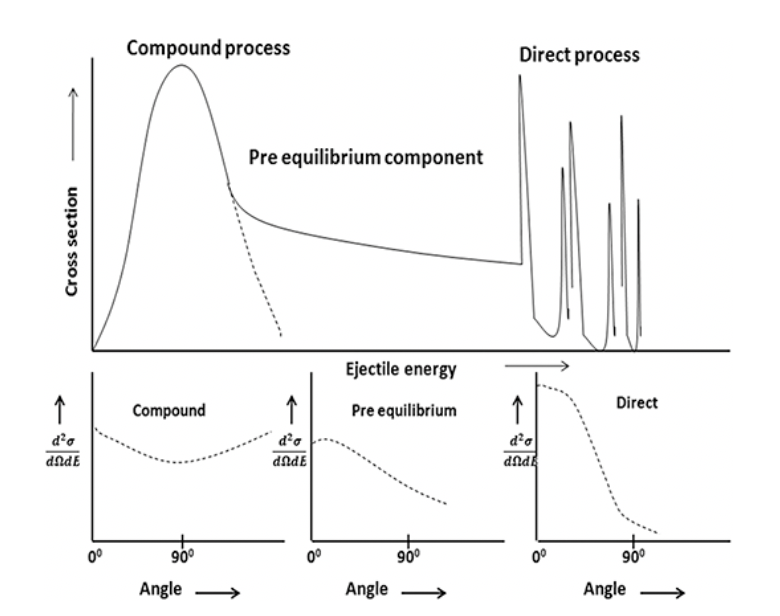
\includegraphics[width=0.45\linewidth]{Images/Energy_Spectrum_Double_cross-section.png}
\caption{Schematic energy spectrum showing typical contributions from compound, pre-equilibrium, and direct-like mechanisms and the typical angular distributions for each component. Adapted from \cite{preeq_image}.}
\label{fig:mechanisms_schematic}
\end{figure}

\section{Methodology}

In this work, TALYS simulations were compared with experimental outgoing-particle energy spectra from EXFOR. The main objective was to evaluate how well TALYS reproduces the measured light-ion spectra and to investigate the sensitivity of the results to different pre-equilibrium model settings. The reactions studied were:

\begin{itemize}
\item proton production, ((n,px)), on selected targets, including \ce{^{28}Si}, \ce{^{56}Fe}, \ce{^{52}Cr}, \ce{^{51}V}, and \ce{^{59}Co};
\item deuteron production, ((n,dx)), on \ce{^{28}Si};
\item alpha production, ((n,\alpha x)), on \ce{^{28}Si}.
\end{itemize}

For each reaction case, TALYS calculations were performed for the incident neutron energies available in the selected EXFOR datasets, or for a representative subset of those energies when the dataset contained a large number of points. The outgoing-particle energy is denoted by (E_{\mathrm{out}}), and the calculated spectra were compared with the corresponding EXFOR energy-differential cross sections.

To study the sensitivity of the calculated spectra to the treatment of pre-equilibrium emission, four TALYS calculations were performed for each reaction case, corresponding to \texttt{preeqmode = 1--4}. According to the TALYS manual, these options select different models for pre-equilibrium reactions, ranging from exciton-model calculations with different treatments of transition rates to a multi-step direct/compound model \cite{koning2025talys}. In this work, the four calculations are labelled as \texttt{preeq1}, \texttt{preeq2}, \texttt{preeq3}, and \texttt{preeq4}. All other input conditions were kept fixed, so that differences between the spectra could be attributed mainly to the selected pre-equilibrium model.

\begin{table}[H]
\centering
\caption{TALYS pre-equilibrium models compared in this work. Definitions follow the TALYS manual \cite{koning2025talys}.}
\label{tab:preeq-configurations}
\begin{tabular}{c c p{0.62\textwidth}}
\hline
\textbf{Label used in this work} & \textbf{TALYS keyword} & \textbf{Model definition} \
\hline
\texttt{preeq1} & \texttt{preeqmode 1} & Exciton model: analytical transition rates with energy-dependent matrix element. \

\texttt{preeq2} & \texttt{preeqmode 2} & Exciton model: numerical transition rates with energy-dependent matrix element. \

\texttt{preeq3} & \texttt{preeqmode 3} & Exciton model: numerical transition rates with optical model for collision probability. \

\texttt{preeq4} & \texttt{preeqmode 4} & Multi-step direct/compound model. \
\hline
\end{tabular}
\end{table}


The comparison was based on both qualitative and quantitative criteria. First, the TALYS total spectra were plotted together with the EXFOR data in linear scale, in order to compare the overall shape, the peak position, and the peak magnitude. The same comparison was also shown in logarithmic scale, which makes it easier to inspect the low-cross-section region and the high-(E_{\mathrm{out}}) tail.

Second, the TALYS spectra were compared with EXFOR through a point-by-point ratio. Since the TALYS output and the EXFOR data are not always given at exactly the same outgoing energies, the TALYS total spectrum was interpolated at the EXFOR (E_{\mathrm{out}}) values. The ratio was then calculated as

\begin{equation}
R(E_{\mathrm{out}}) =
\frac{\left(\mathrm{d}\sigma/\mathrm{d}E\right)*{\mathrm{TALYS}}(E*{\mathrm{out}})}
{\left(\mathrm{d}\sigma/\mathrm{d}E\right)*{\mathrm{EXFOR}}(E*{\mathrm{out}})} .
\label{eq:ratio}
\end{equation}

A value (R(E_{\mathrm{out}}) \simeq 1) indicates good agreement between TALYS and EXFOR at that outgoing energy. Values above 1 indicate that TALYS overpredicts the experimental data, while values below 1 indicate an underprediction. The ratio plot is especially useful when the total spectra appear visually similar, because it makes systematic deviations easier to identify.

Finally, for the selected pre-equilibrium mode in each case, the TALYS spectrum was decomposed into its main reaction-mechanism components. This made it possible to identify which parts of the spectrum are mainly associated with compound emission, pre-equilibrium emission, direct-like processes, or multiple pre-equilibrium emission. In general, the low-(E_{\mathrm{out}}) peak is expected to be more strongly associated with compound-nucleus evaporation, while the shoulder and high-(E_{\mathrm{out}}) tail are more sensitive to pre-equilibrium and direct-like contributions.

Each diagnostic figure therefore contains four panels: the total TALYS--EXFOR comparison in linear scale, the same comparison in logarithmic scale, the ratio (R(E_{\mathrm{out}})) for all four \texttt{preeqmode} options, and the mechanism decomposition for the selected mode. The best-performing mode was chosen by considering the total spectrum, the ratio behaviour, and the physical interpretation of the component decomposition. Particular attention was given to the shoulder and high-energy tail, because these regions are often more sensitive to the pre-equilibrium treatment than the main evaporation peak.

In the logarithmic plots, very small TALYS values near the numerical or physical end of the spectrum were interpreted with caution. These regions can visually exaggerate differences between modes, especially when EXFOR has few or no data points there. For this reason, the final assessment focused mainly on the outgoing-energy interval where experimental data are available and physically meaningful comparisons can be made.

\section{Results}

\subsection{Proton Production}

\subsubsection*{\ce{^{28}Si}, Benck, 22807.012}

For this dataset, TALYS simulations were analysed in the incident-energy interval $E_n \in [28.0,50.0]\,\mathrm{MeV}$. The same comparison methodology was applied at each energy and for each pre-equilibrium option (\texttt{preeqmode}=1--4). Following the procedure described above, the following study was conducted.

\Epar{$E_n=28.0$ MeV}

\begin{figure}[H]
    \centering
    
\includegraphics[width=\textwidth]{Images/Proton/Benck/proton/EN28.0_00_2x2_diagnostics_28Si_np_Benck_22807_012.png}
    \caption{Diagnostic comparison for proton production from \ce{^{28}Si}, Benck dataset 22807.012, at $E_n=28.0$ MeV.}
    \label{fig:benck-en28-p-diagnostics}
\end{figure}

Observing \cref{fig:benck-en28-p-diagnostics}, one can see that the best approximation to the EXFOR data is given mainly by preeq mode 1 or 2, as they overlap the most with the experimental points. However, it is not straightforward to decide between them for one striking reason: the EXFOR data only starts at an outgoing energy of about $5$ MeV, which is not surprising given its experimental nature and the use of detectors that are harder to work with at lower energies. Looking at the same comparison with a logarithmic $y$-axis helps to visualise the tail behaviour, but differences appear only where the cross section becomes very small, or where EXFOR has no points, which should be taken with a grain of salt.

The ratio panel shows that the selected mode reproduces the bulk of the spectrum with relatively small deviations around $R\simeq 1$, while making it easier to identify where the simulation over- or underpredicts the data. In particular, the deviations are smaller in the mid-energy region, whereas larger excursions appear closer to the edges of the measured range. The components panel indicates that the low-$E_{\mathrm{out}}$ peak is dominated by the compound contribution, while pre-equilibrium mainly supports the shoulder and the tail.

\Epar{$E_n=40.0$ MeV}

\begin{figure}[H]
    \centering
    
\includegraphics[width=\textwidth]{Images/Proton/Benck/proton/EN40.0_00_2x2_diagnostics_28Si_np_Benck_22807_012.png}
    \caption{Diagnostic comparison for proton production from \ce{^{28}Si}, Benck dataset 22807.012, at $E_n=40.0$ MeV.}
    \label{fig:benck-en40-p-diagnostics}
\end{figure}

In \cref{fig:benck-en40-p-diagnostics}, one is once again torn between modes 1 and 2, since they overlap most of the experimental spectrum, while modes 3 and 4 deviate more visibly in the shoulder/tail. The main qualitative difference observed between the remaining modes is that mode 4 tends to provide the largest cross section, especially around the peak/shoulder region. The logarithmic view is again important to inspect the tail, where the curves can separate even when the linear plot makes them look similar.

Comparing the calculated ratios, preeq mode 1 stands out as the most stable configuration for this dataset, even if it still shows a non-negligible error magnitude in some regions. The ratio tends to stay closer to 1 at lower and intermediate outgoing energies, and then progressively deviates as $E_{\mathrm{out}}$ increases, which suggests that the tail is the most sensitive part of the spectrum at this incident energy. The components panel supports this view by showing a stronger role of pre-equilibrium in the shoulder and tail compared with the lowest $E_{\mathrm{out}}$ region, which remains dominated by the compound component.

\Epar{$E_n=50.0$ MeV}

\begin{figure}[H]
    \centering
    
\includegraphics[width=\textwidth]{Images/Proton/Benck/proton/EN50.0_00_2x2_diagnostics_28Si_np_Benck_22807_012.png}
    \caption{Diagnostic comparison for proton production from \ce{^{28}Si}, Benck dataset 22807.012, at $E_n=50.0$ MeV.}
    \label{fig:benck-en50-p-diagnostics}
\end{figure}

The same thought process is once again repeated. Modes 1 and 2 remain the closest to the experimental points in the main part of the spectrum, while the log-scale panel becomes especially useful to check whether the tail is too soft or too hard and where the effective cut-off appears. At this energy, the outgoing-energy distribution extends further, and therefore the high-$E_{\mathrm{out}}$ region becomes increasingly important for distinguishing between modes.

The ratio and component panels confirm the overall behaviour seen at lower energies: the compound component dominates the low-$E_{\mathrm{out}}$ peak, while pre-equilibrium provides the main support to the shoulder and the tail. The remaining discrepancies are more visible towards the high-$E_{\mathrm{out}}$ end of the spectrum, indicating that this is the region where the model choice matters the most for this dataset.

\subsubsection*{\ce{^{28}Si}, Bateman, 13740.005}

EXFOR provides incident energies in the interval $E_n\in[4,51]\,\mathrm{MeV}$. To facilitate comparison with the Benck dataset, we restrict the TALYS calculations to
$E_n=\{28.0,\,30.0,\,35.0,\,40.0,\,45.0,\,50.0\}\,\mathrm{MeV}$.
To keep the report concise and avoid repetition, only $E_n=28.0$, 40.0, and 50.0~MeV are shown here; the remaining incident energies follow the same reasoning and are provided in Appendix~A.

\Epar{$E_n=28.0$ MeV}

\begin{figure}[H]
    \centering
    
\includegraphics[width=\textwidth]{Images/Proton/Bateman/proton/EN28.0_00_2x2_diagnostics_28Si_np_Bateman_13740_005.png}
    \caption{Diagnostic comparison for proton production from \ce{^{28}Si}, Bateman dataset 13740.005, at $E_n=28.0$ MeV.}
    \label{fig:bateman-en28-p-diagnostics}
\end{figure}

Observing the totals comparison in \cref{fig:bateman-en28-p-diagnostics}, the four modes are close in the peak region, while differences become clearer in the shoulder and tail. The ratio panel shows that after the first points, which have larger uncertainties, the ratio remains reasonably close to $R\simeq 1$ across most of the measured outgoing-energy range, with the largest deviations concentrated at the highest $E_{\mathrm{out}}$ values.

\Epar{$E_n=40.0$ MeV}

\begin{figure}[H]
    \centering
    
\includegraphics[width=\textwidth]{Images/Proton/Bateman/proton/EN40.0_00_2x2_diagnostics_28Si_np_Bateman_13740_005.png}
    \caption{Diagnostic comparison for proton production from \ce{^{28}Si}, Bateman dataset 13740.005, at $E_n=40.0$ MeV.}
    \label{fig:bateman-en40-p-diagnostics}
\end{figure}

At $E_n=40.0$ MeV, the totals overlap strongly near the peak and separate more in the shoulder and tail, which allows us to rule out pre-equilibrium modes 3 and 4. For the selected mode, the ratio starts at a relatively high value at low outgoing energies and then settles closer to 1; deviations grow again toward higher $E_{\mathrm{out}}$, indicating that the tail is the most discriminating region.

\Epar{$E_n=50.0$ MeV}

\begin{figure}[H]
    \centering
    
\includegraphics[width=\textwidth]{Images/Proton/Bateman/proton/EN50.0_00_2x2_diagnostics_28Si_np_Bateman_13740_005.png}
    \caption{Diagnostic comparison for proton production from \ce{^{28}Si}, Bateman dataset 13740.005, at $E_n=50.0$ MeV.}
    \label{fig:bateman-en50-p-diagnostics}
\end{figure}

At $E_n=50.0$ MeV, the same overall pattern is observed. Overall, the agreement improves with increasing incident energy $E_n$: in this case the ratio remains closer to 1 up to about $E_{\mathrm{out}}\approx 30$ MeV. For Bateman (13740.005), the mode selection is driven less by the peak region, where the totals often overlap, and more by the shoulder/tail behaviour, which is consistently highlighted by the ratio plots across the analysed incident energies.

\subsubsection*{\ce{^{56}Fe}, Slypen, 22884.015}

The Slypen dataset provides an additional proton-production comparison for iron. The same diagnostic representation is used here, allowing the total spectra, ratio behaviour, and model-component decomposition to be assessed in a single figure for each incident energy.

\Epar{$E_n=28.5$ MeV}

\begin{figure}[H]
    \centering
    
\includegraphics[width=\textwidth]{Images/Proton/Slypen/proton/EN28.5_00_2x2_diagnostics_56Fe_np_Slypen_22884_015.png}
    \caption{Diagnostic comparison for proton production from \ce{^{56}Fe}, Slypen dataset 22884.015, at $E_n=28.5$ MeV.}
    \label{fig:slypen-en28p5-p-diagnostics}
\end{figure}

As shown in \cref{fig:slypen-en28p5-p-diagnostics}, the main peak is reasonably well reproduced by the TALYS totals, although the different pre-equilibrium modes lead to visible differences in both peak height and shoulder behaviour. The ratio panel indicates that the selected mode gives the best compromise over the measured range, while the high-energy tail remains difficult to reproduce exactly. The component decomposition shows that the low-energy peak receives a strong compound contribution, while the shoulder and tail are mainly constrained by pre-equilibrium emission.

\Epar{$E_n=34.5$ MeV}

\begin{figure}[H]
    \centering
    
\includegraphics[width=\textwidth]{Images/Proton/Slypen/proton/EN34.5_00_2x2_diagnostics_56Fe_np_Slypen_22884_015.png}
    \caption{Diagnostic comparison for proton production from \ce{^{56}Fe}, Slypen dataset 22884.015, at $E_n=34.5$ MeV.}
    \label{fig:slypen-en34p5-p-diagnostics}
\end{figure}

At $E_n=34.5$ MeV, the same general behaviour is observed. The TALYS curves reproduce the order of magnitude of the EXFOR data, but the ratio panel shows that the agreement varies across the outgoing-energy range. In particular, the shoulder and high-energy tail remain the most informative regions for distinguishing between pre-equilibrium modes. The remaining Slypen incident energies are shown in Appendix~A.

\subsection{Deuteron Production}

Compared with proton production, deuteron emission is more difficult to reproduce because the emitted particle is composite. In addition to compound and pre-equilibrium emission, the component decompositions may include contributions such as stripping, knock-out and break-up. As a result, the calculated deuteron spectra show more structure than the proton spectra, especially in the intermediate- and high-outgoing-energy regions. For this reason, the mode selection is again based mainly on the shoulder and high-energy tail, rather than only on the low-energy evaporation peak.

\subsubsection*{\ce{^{28}Si}, Benck, 22807.027}

\Epar{$E_n=28.5$ MeV}

\begin{figure}[H]
    \centering
    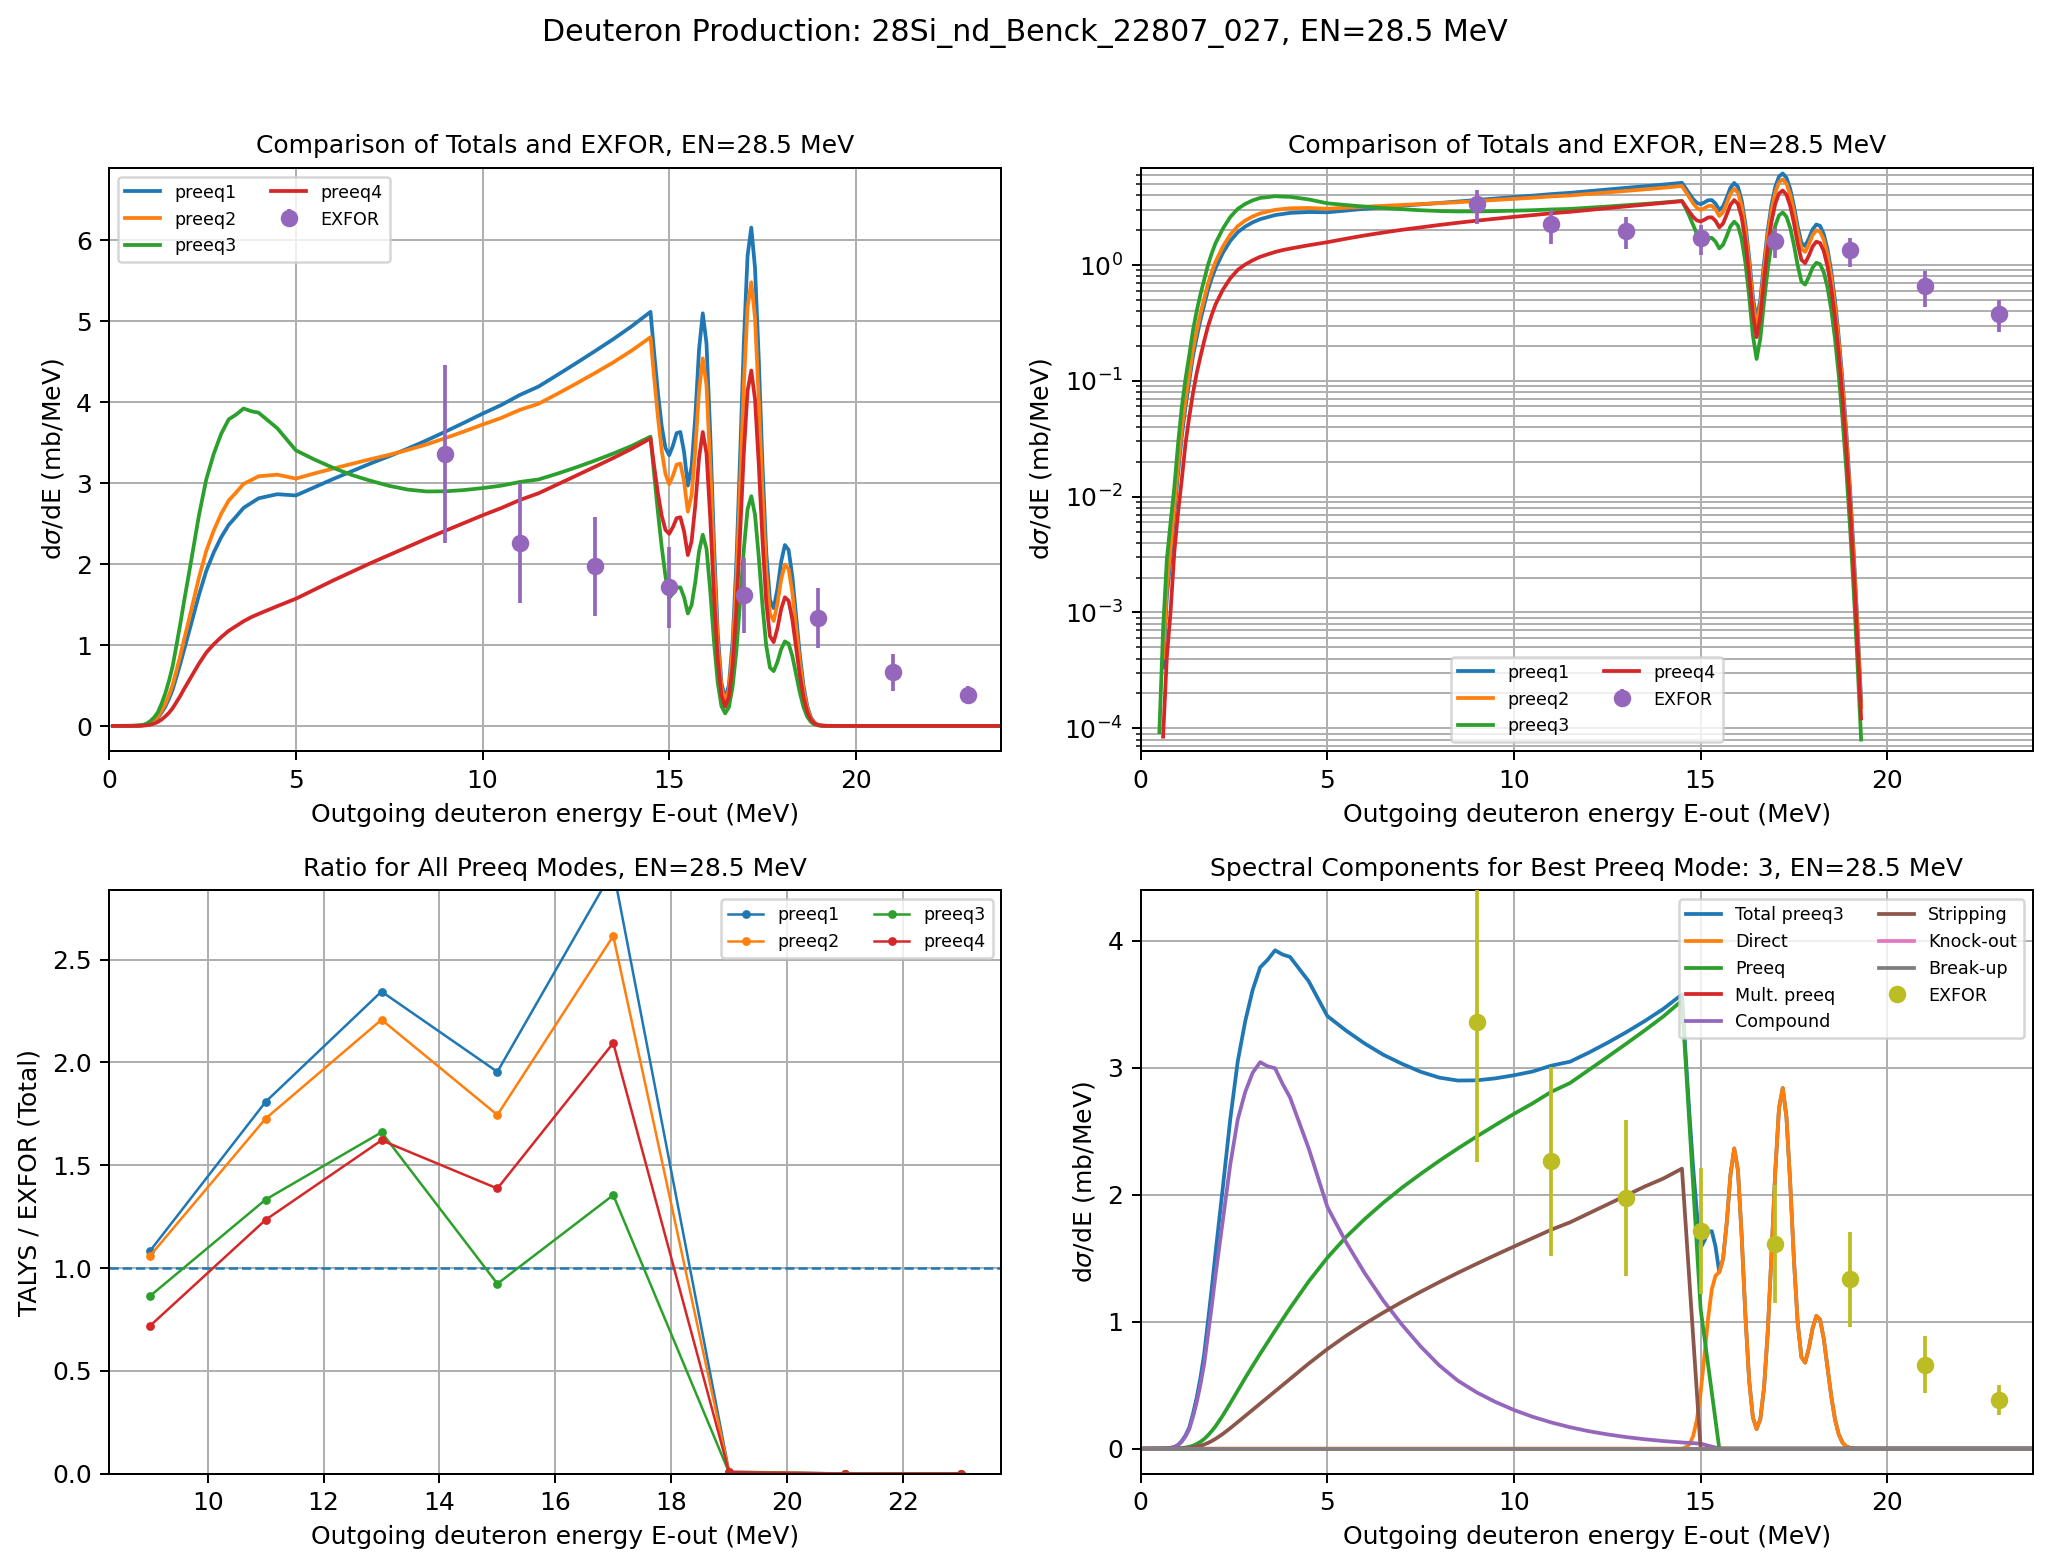
\includegraphics[width=\textwidth]{Images/EN28.5_00_2x2_diagnostics_28Si_nd_Benck_22807_027.png}
    \caption{Diagnostic panels for deuteron production on \ce{^{28}Si} using the Benck EXFOR dataset 22807.027 at $E_n=28.5$ MeV. The decomposition panel corresponds to the selected mode, \texttt{preeqmode=3}.}
    \label{fig:benck-en28p5-d-diagnostics}
\end{figure}

As shown in \cref{fig:benck-en28p5-d-diagnostics}, the deuteron spectrum is less smooth than the corresponding proton-production spectra. The four \texttt{preeqmode} options separate not only in the tail, but also through narrow structures in the mid-to-high outgoing-energy region. This behaviour is consistent with the more complex nature of composite-particle emission, where several mechanisms can contribute to the calculated spectrum.

Among the four options, \texttt{preeqmode=3} gives the most reasonable overall compromise over the better-populated part of the experimental spectrum. The logarithmic panel highlights an important limitation: the TALYS total decreases abruptly around $E_{\mathrm{out}}\approx 19$--20~MeV, while EXFOR still reports non-zero values beyond that region.

The ratio panel confirms this behaviour. After the first points, the ratio fluctuates around $R\simeq 1$, although there is some overprediction in the mid-energy region. The most significant discrepancy occurs above $E_{\mathrm{out}}\sim 19$ MeV, where the TALYS total becomes almost zero while the EXFOR data remain non-zero. This indicates that, for this incident energy, the model has difficulty reproducing the fastest emitted deuterons. The component decomposition shows that, beyond the compound contribution at low $E_{\mathrm{out}}$, the spectrum receives important support from non-compound mechanisms and pre-equilibrium emission in the shoulder region.

\Epar{$E_n=41.0$ MeV}

\begin{figure}[H]
    \centering
    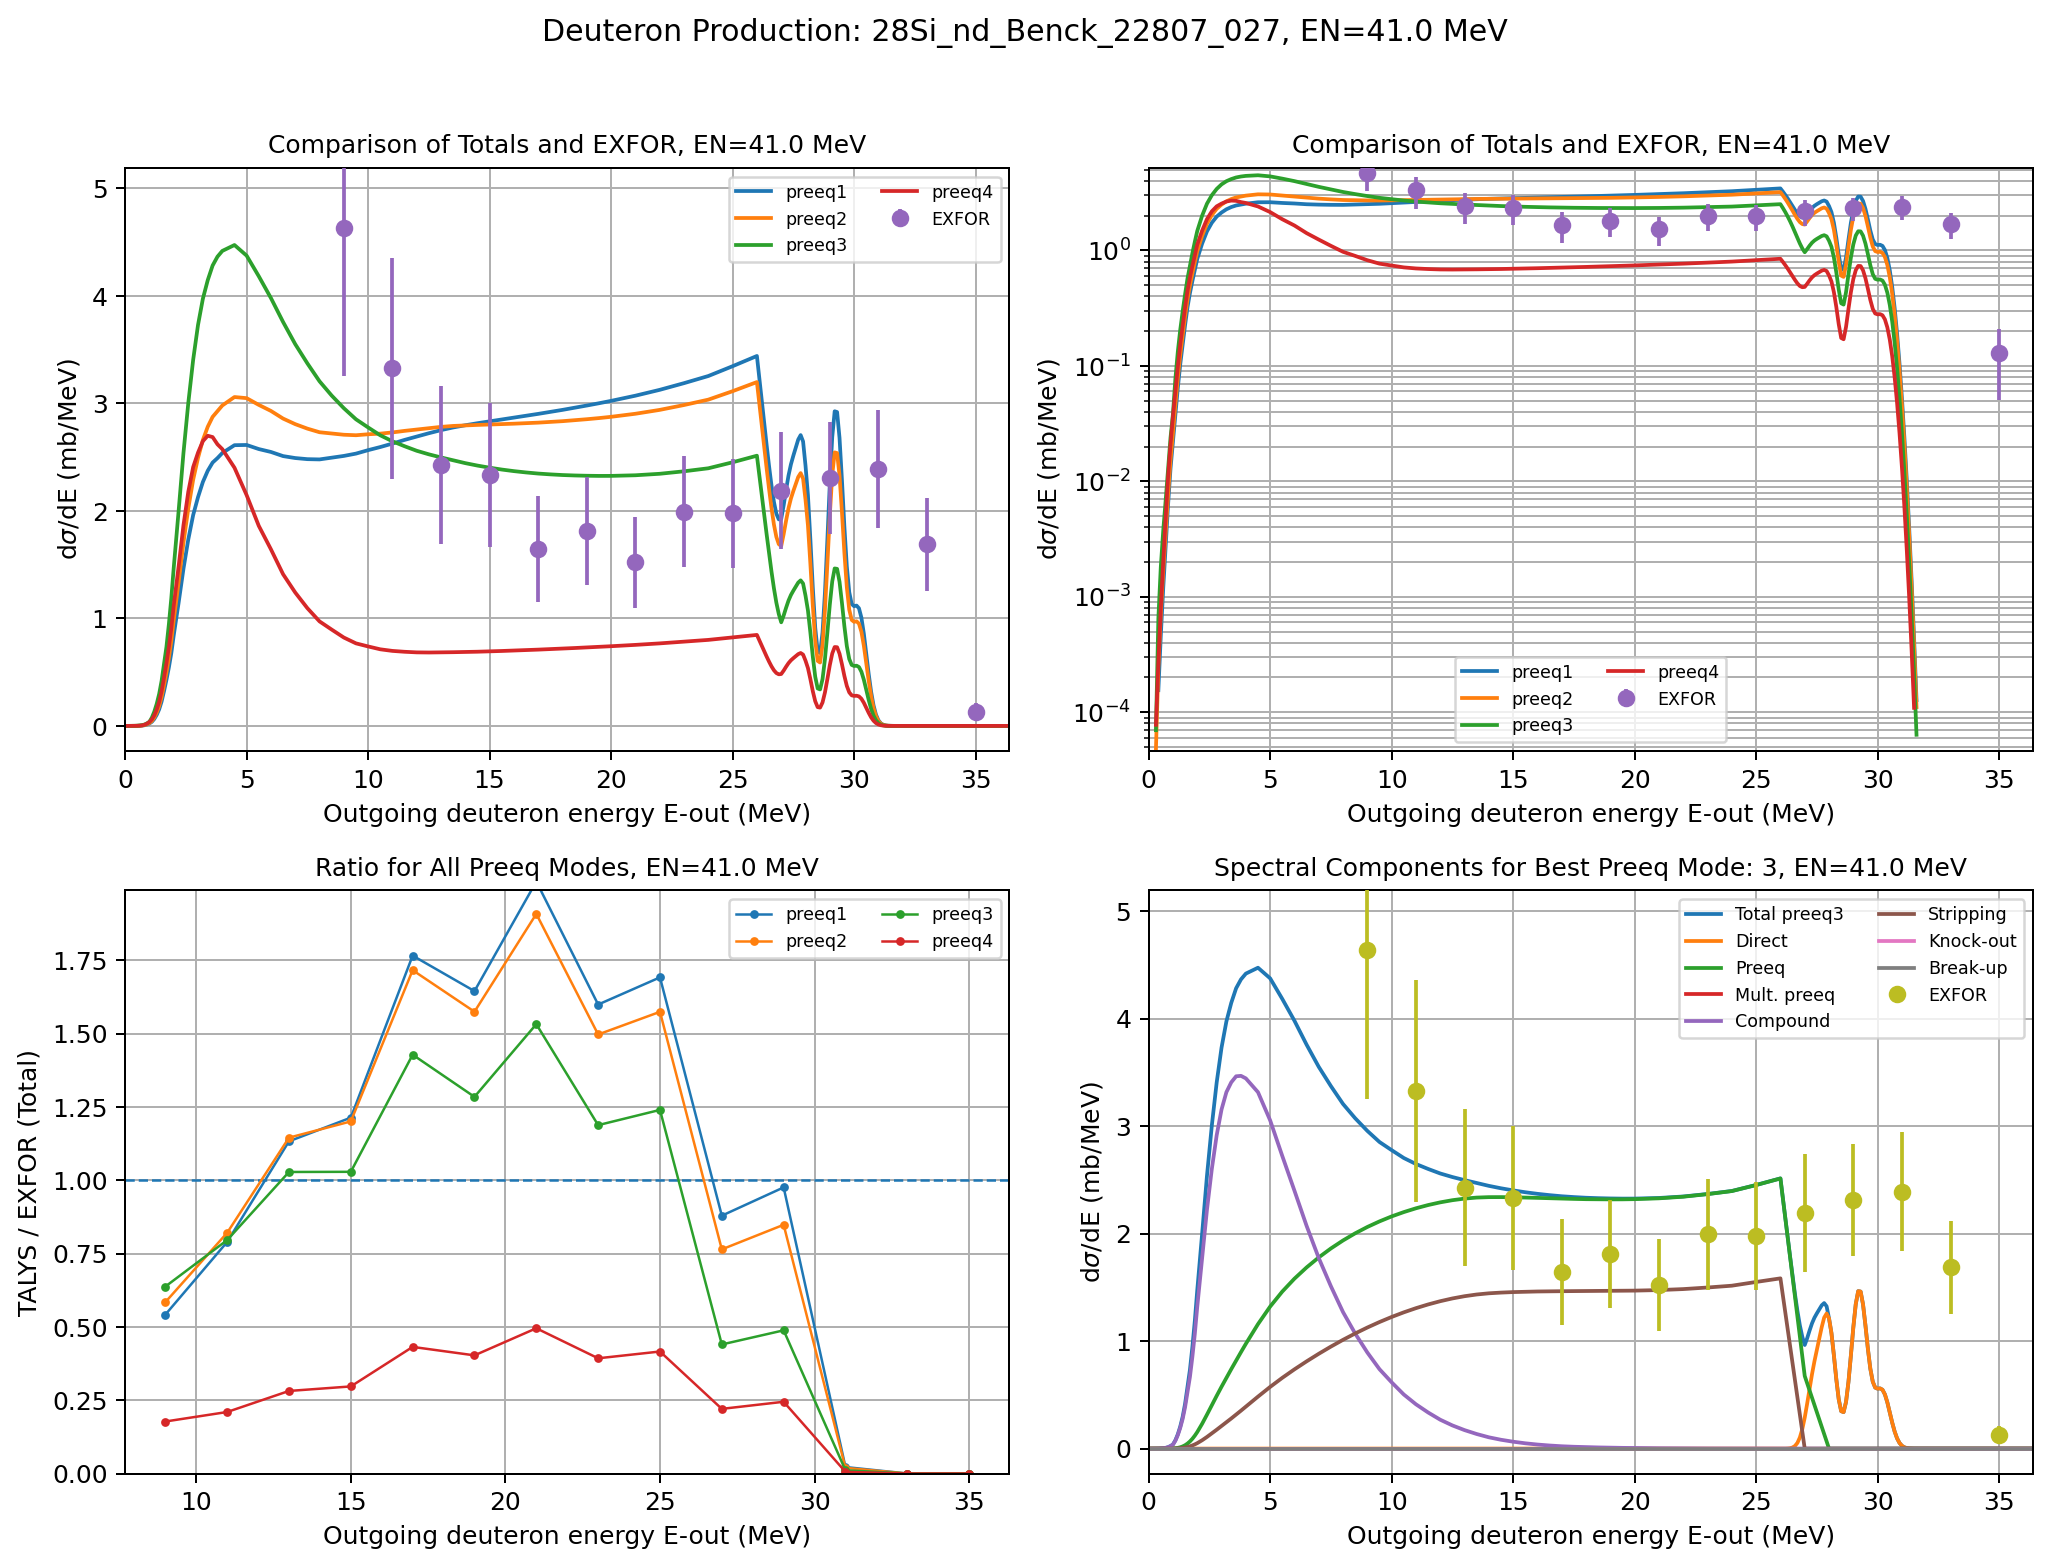
\includegraphics[width=\textwidth]{Images/EN41.0_00_2x2_diagnostics_28Si_nd_Benck_22807_027.png}
    \caption{Diagnostic panels for deuteron production on \ce{^{28}Si} using the Benck EXFOR dataset 22807.027 at $E_n=41.0$ MeV. The decomposition panel corresponds to the selected mode, \texttt{preeqmode=3}.}
    \label{fig:benck-en41-d-diagnostics}
\end{figure}

At $E_n=41.0$ MeV, shown in \cref{fig:benck-en41-d-diagnostics}, the agreement between TALYS and EXFOR improves compared with the lower incident energy. The calculated spectra still show visible structures in the shoulder and high-energy region, but the overall shape follows the experimental trend more coherently.

The ratio panel provides a clearer view of this improvement. Although the ratio still deviates from $R=1$, the decrease is less abrupt than at $E_n=28.5$ MeV. The TALYS prediction only approaches zero above approximately $E_{\mathrm{out}}\sim 30$ MeV. This means that, as the incident energy increases, the region where TALYS remains non-zero extends to higher outgoing energies. Nevertheless, the high-energy tail remains the most problematic region, and \texttt{preeqmode=3} gives the best overall compromise among the tested modes.

\Epar{$E_n=49.0$ MeV}

\begin{figure}[H]
    \centering
    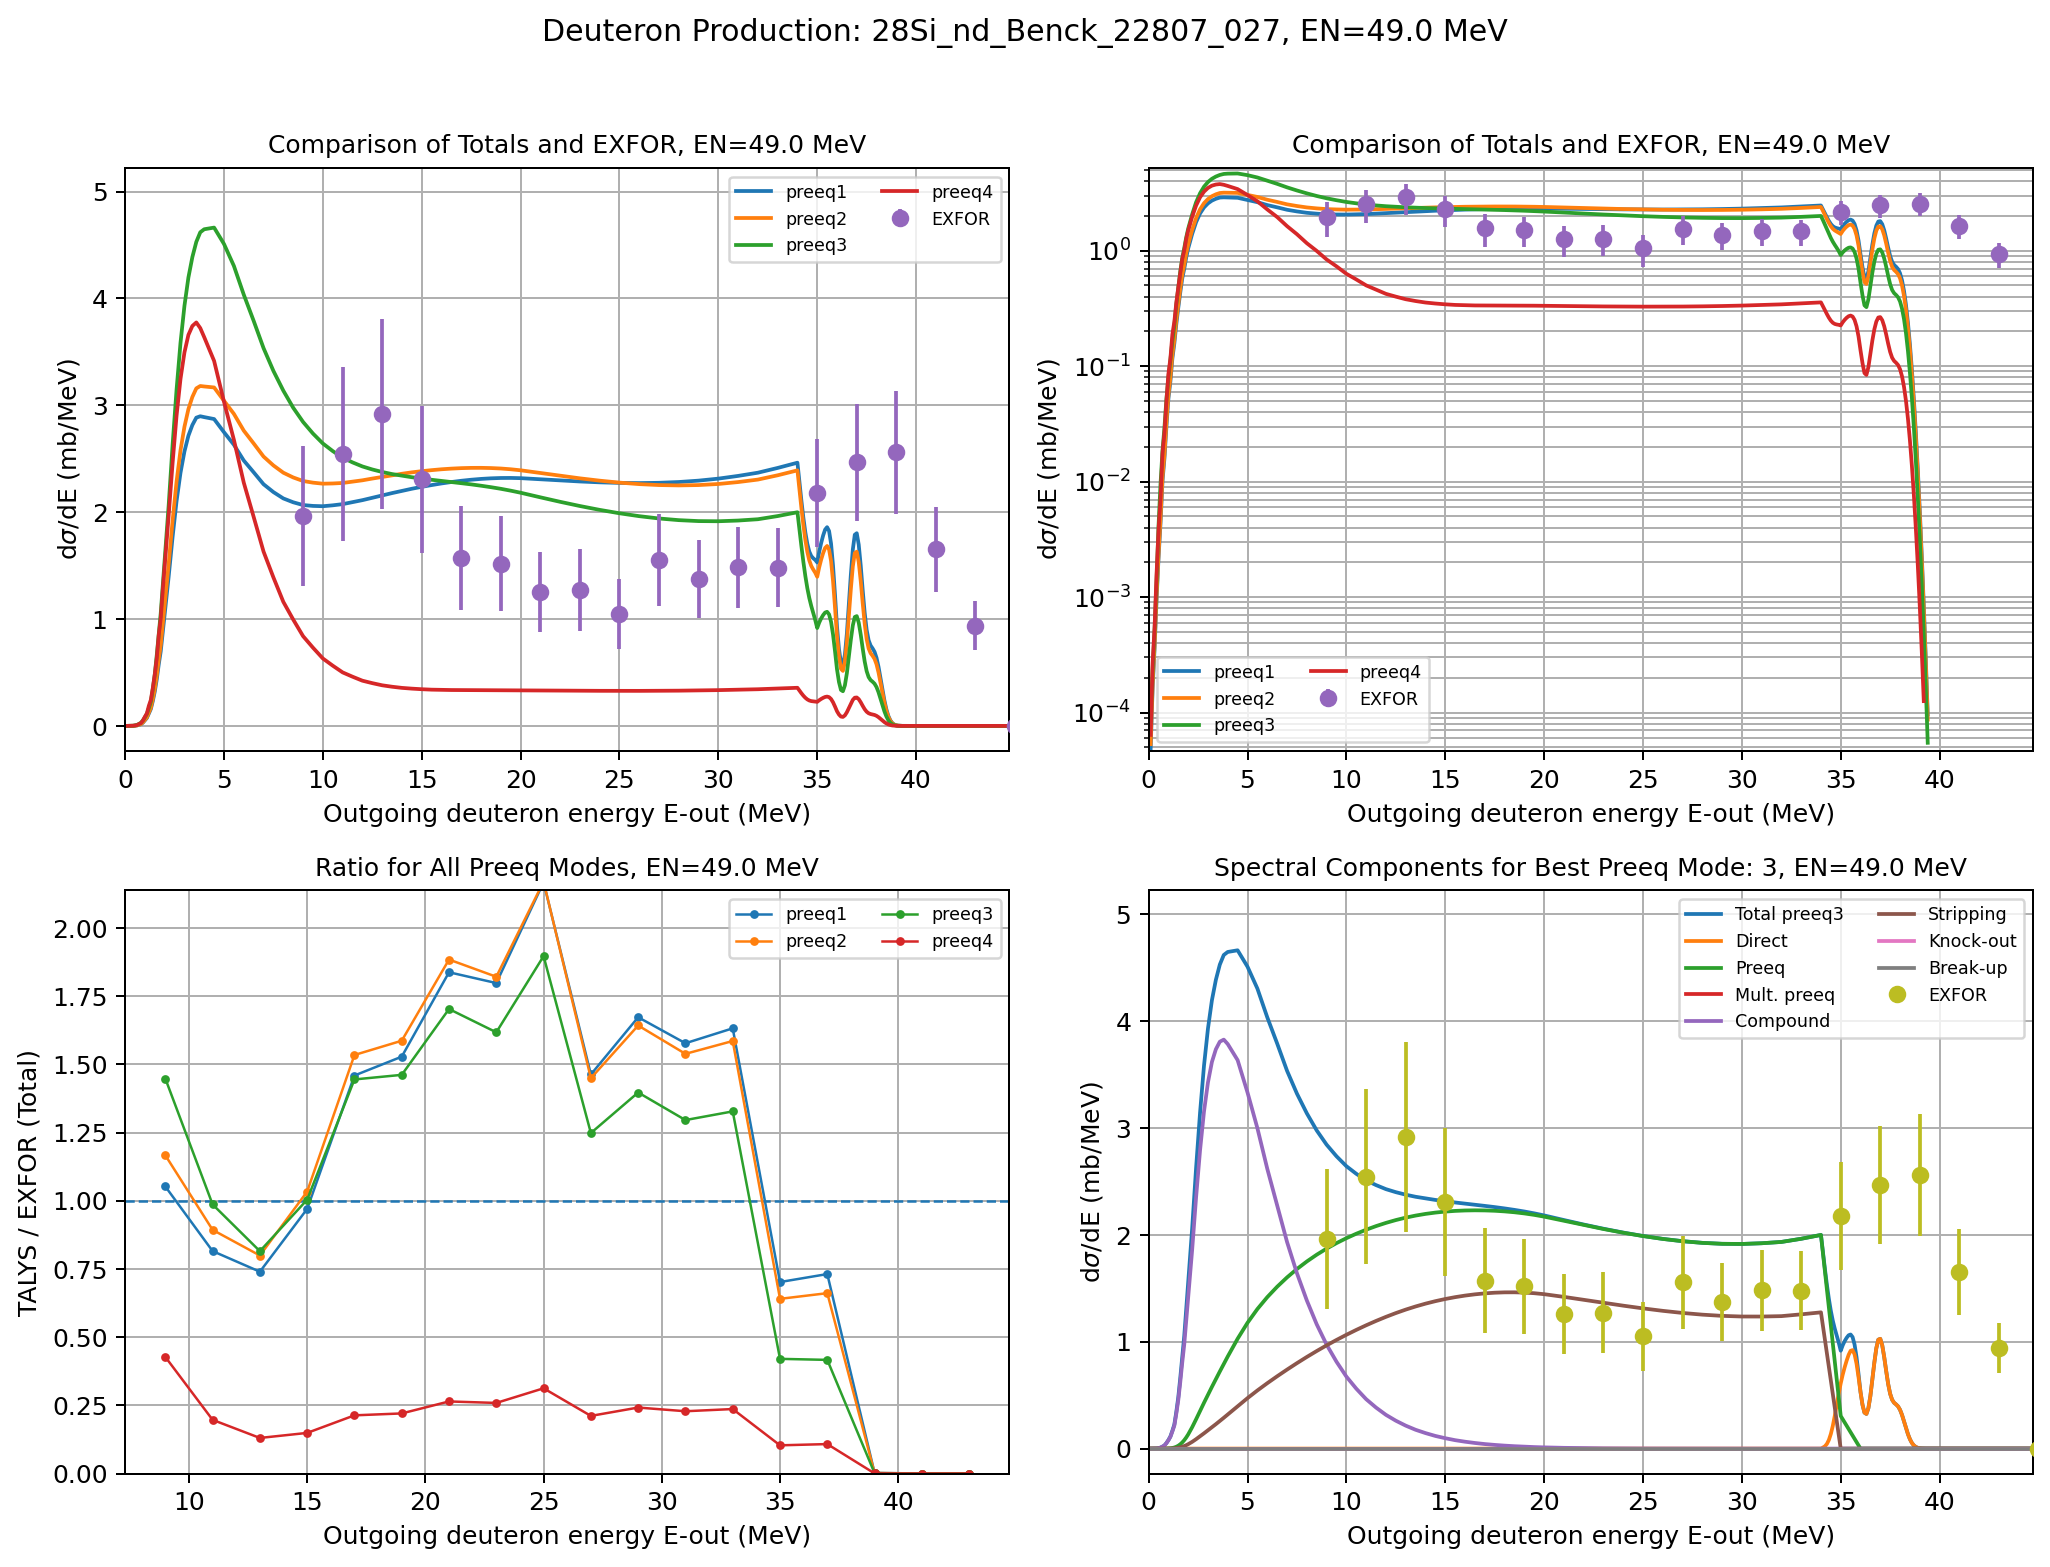
\includegraphics[width=\textwidth]{Images/EN49.0_00_2x2_diagnostics_28Si_nd_Benck_22807_027.png}
    \caption{Diagnostic panels for deuteron production on \ce{^{28}Si} using the Benck EXFOR dataset 22807.027 at $E_n=49.0$ MeV. The decomposition panel corresponds to the selected mode, \texttt{preeqmode=3}.}
    \label{fig:benck-en49-d-diagnostics}
\end{figure}

At $E_n=49.0$ MeV, shown in \cref{fig:benck-en49-d-diagnostics}, the comparison again improves in the sense that the TALYS prediction remains non-zero over a larger outgoing-energy range. The overall overlap between TALYS and EXFOR is better than at lower incident energies, although sizeable discrepancies and experimental error bars remain.

The ratio panel shows that the TALYS prediction falls to nearly zero only around $E_{\mathrm{out}}\sim 39$ MeV. This is a clear shift toward higher outgoing energy compared with the lower incident-energy cases. However, the ratio also shows larger deviations in some regions, meaning that the high-energy end is still difficult to reproduce accurately. For the Benck deuteron-production dataset, the preferred mode is consistently \texttt{preeqmode=3}, but the agreement is still limited by the treatment of the fastest emitted deuterons.

\subsubsection*{\ce{^{28}Si}, Bateman, 13740.006}

Following the same procedure, this dataset was simulated for
$E_n=\{28.0,\,33.0,\,41.0,\,49.0\}\,\mathrm{MeV}$. To keep the report concise and avoid repetition, only
$E_n=\{28.0,\,41.0,\,49.0\}\,\mathrm{MeV}$ are discussed here; the remaining energy is included in Appendix~A.

\Epar{$E_n=28.0$ MeV}

\begin{figure}[H]
    \centering
    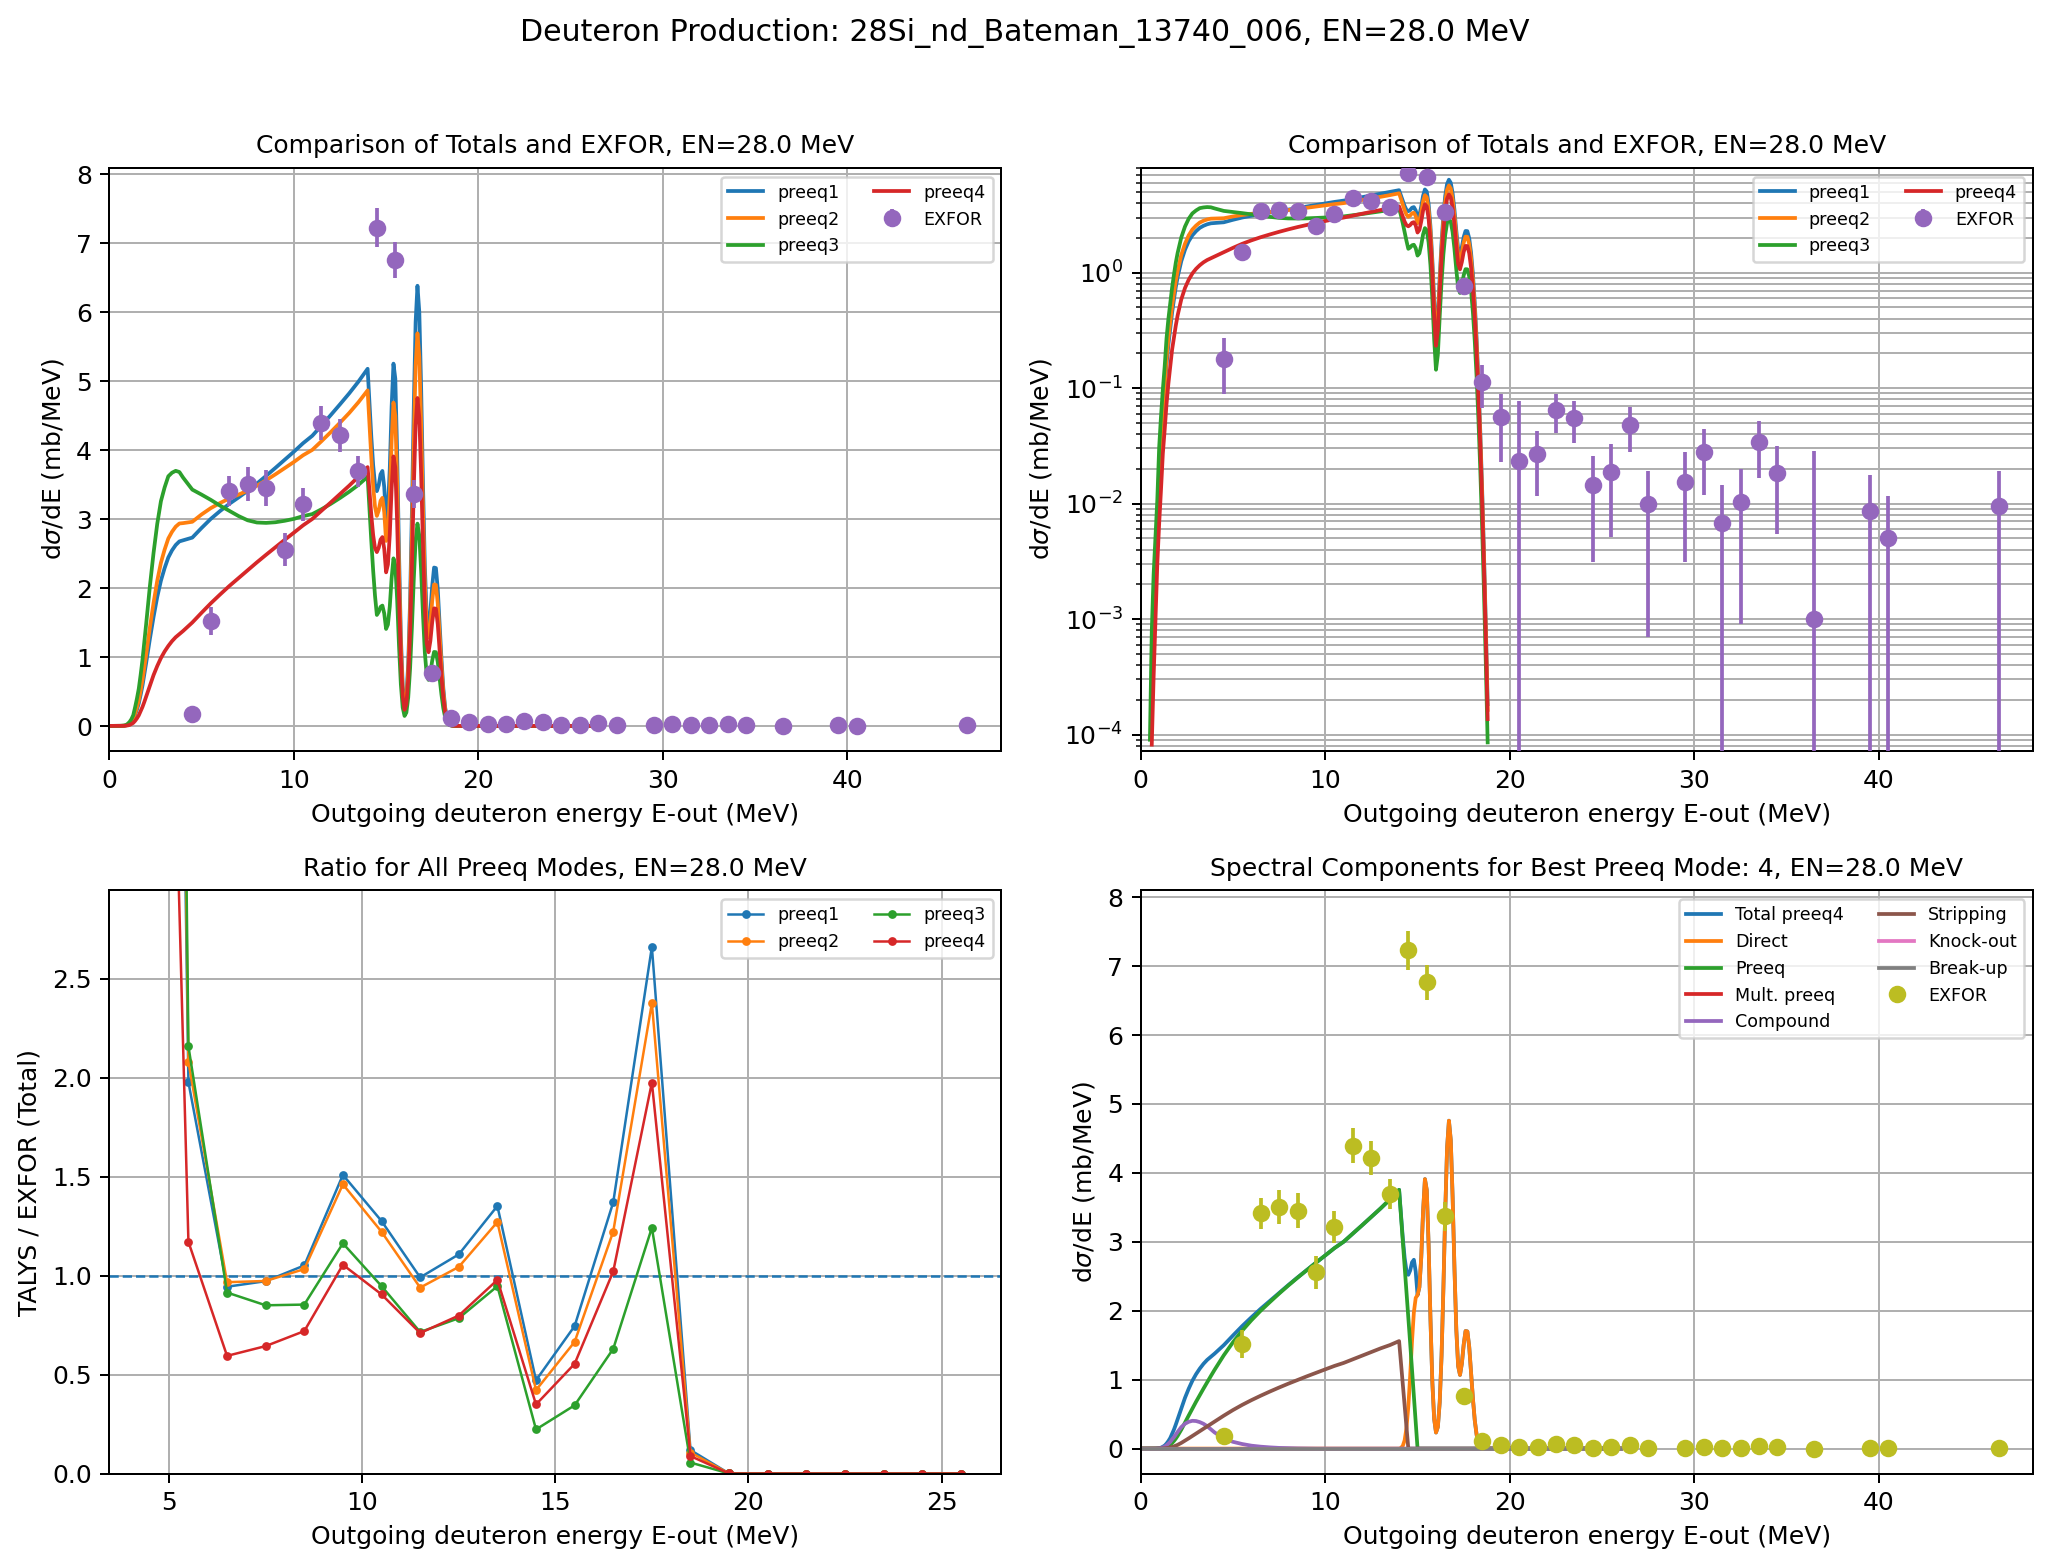
\includegraphics[width=\textwidth]{Images/EN28.0_00_2x2_diagnostics_28Si_nd_Bateman_13740_006.png}
    \caption{Diagnostic panels for deuteron production on \ce{^{28}Si} using the Bateman EXFOR dataset 13740.006 at $E_n=28.0$ MeV. The decomposition panel corresponds to the selected mode, \texttt{preeqmode=4}.}
    \label{fig:bateman-en28-d-diagnostics}
\end{figure}

As shown in \cref{fig:bateman-en28-d-diagnostics}, the Bateman deuteron spectrum also displays a more structured behaviour than the proton-production cases. The \texttt{preeqmode} curves separate not only in the tail, but also through sharp features in the mid-to-high $E_{\mathrm{out}}$ region. Therefore, the mode choice is controlled mainly by the agreement with the EXFOR trend before the TALYS prediction drops to almost zero.

For this incident energy, the selected mode is \texttt{preeqmode=4}. After the first experimental point, which is the most discrepant, the ratio remains closer to $R\simeq 1$ through much of the better-populated region. However, it deviates near the last non-zero TALYS points and eventually collapses to $R\simeq 0$ when the TALYS total becomes almost zero while EXFOR remains non-zero. Thus, at $E_n=28.0$ MeV, the high-energy end is the main limitation of the calculation.

\Epar{$E_n=41.0$ MeV}

\begin{figure}[H]
    \centering
    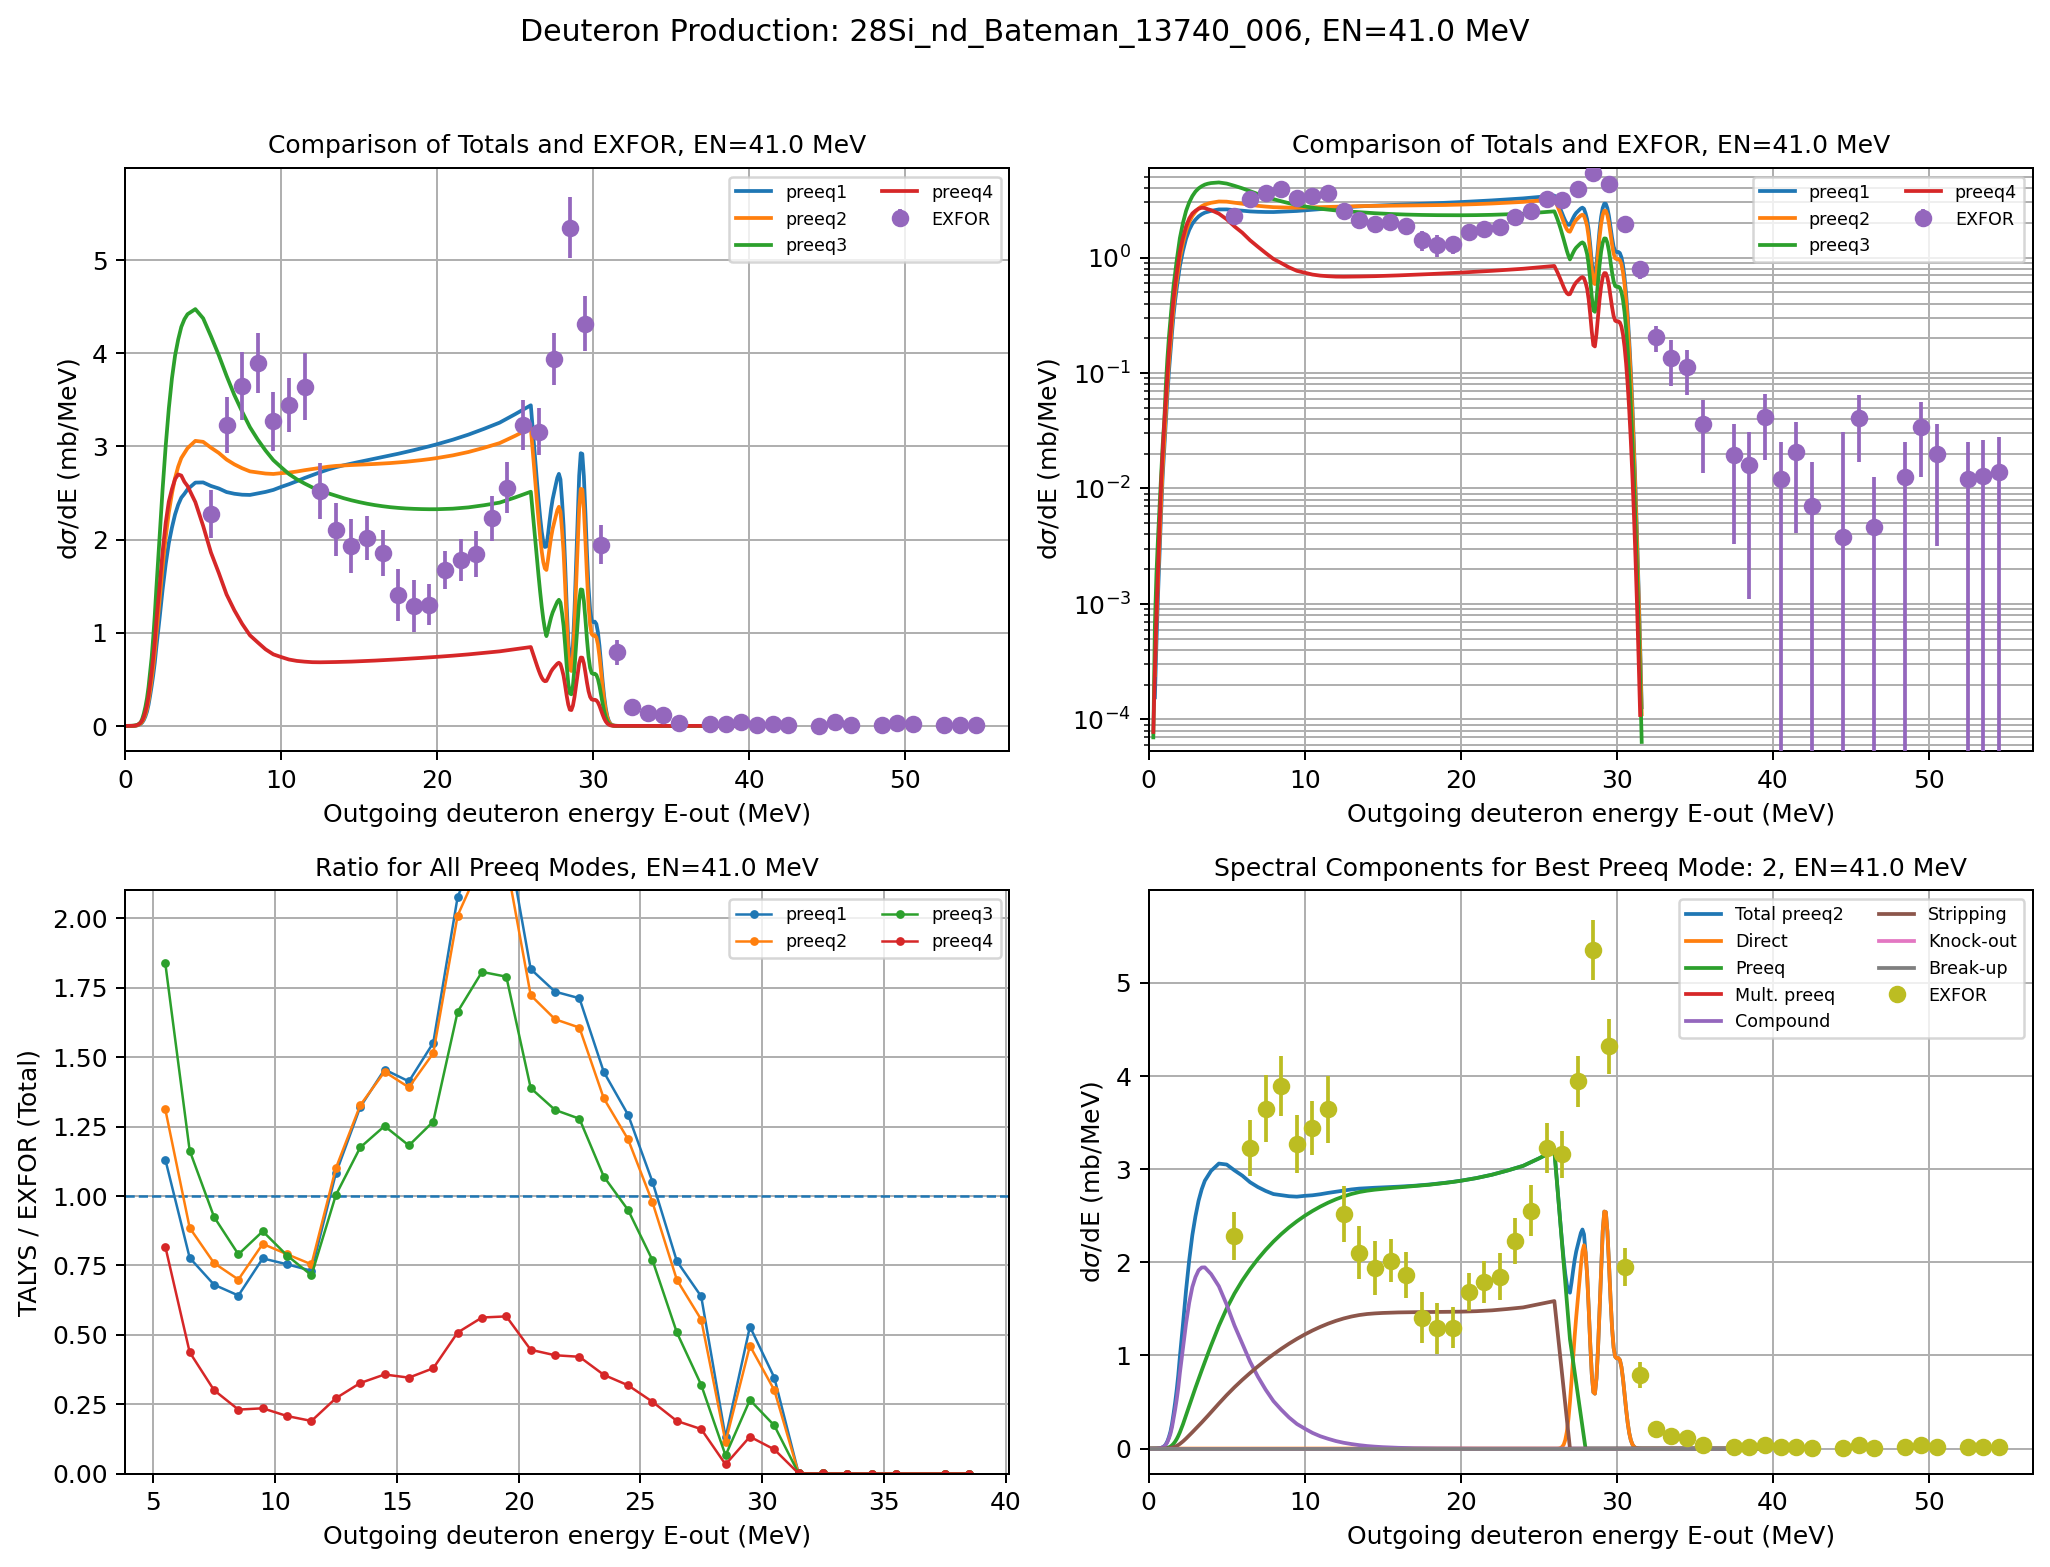
\includegraphics[width=\textwidth]{Images/EN41.0_00_2x2_diagnostics_28Si_nd_Bateman_13740_006.png}
    \caption{Diagnostic panels for deuteron production on \ce{^{28}Si} using the Bateman EXFOR dataset 13740.006 at $E_n=41.0$ MeV. The decomposition panel corresponds to the selected mode, \texttt{preeqmode=2}.}
    \label{fig:bateman-en41-d-diagnostics}
\end{figure}

At $E_n=41.0$ MeV, shown in \cref{fig:bateman-en41-d-diagnostics}, the overall agreement improves, although the calculated spectra still show structured behaviour in the shoulder region. The EXFOR data are followed more coherently over the main part of the measured spectrum, but the high-energy end remains difficult to describe.

For the selected mode, \texttt{preeqmode=2}, the ratio starts close to $R=1$ at lower outgoing energies. It then increases, indicating overprediction in the mid-energy region, before decreasing again and approaching $R\simeq 0$ above $E_{\mathrm{out}}\sim 30$ MeV. Therefore, at this incident energy, the shoulder and high-energy end remain the most sensitive regions for discriminating between modes.

\Epar{$E_n=49.0$ MeV}

\begin{figure}[H]
    \centering
    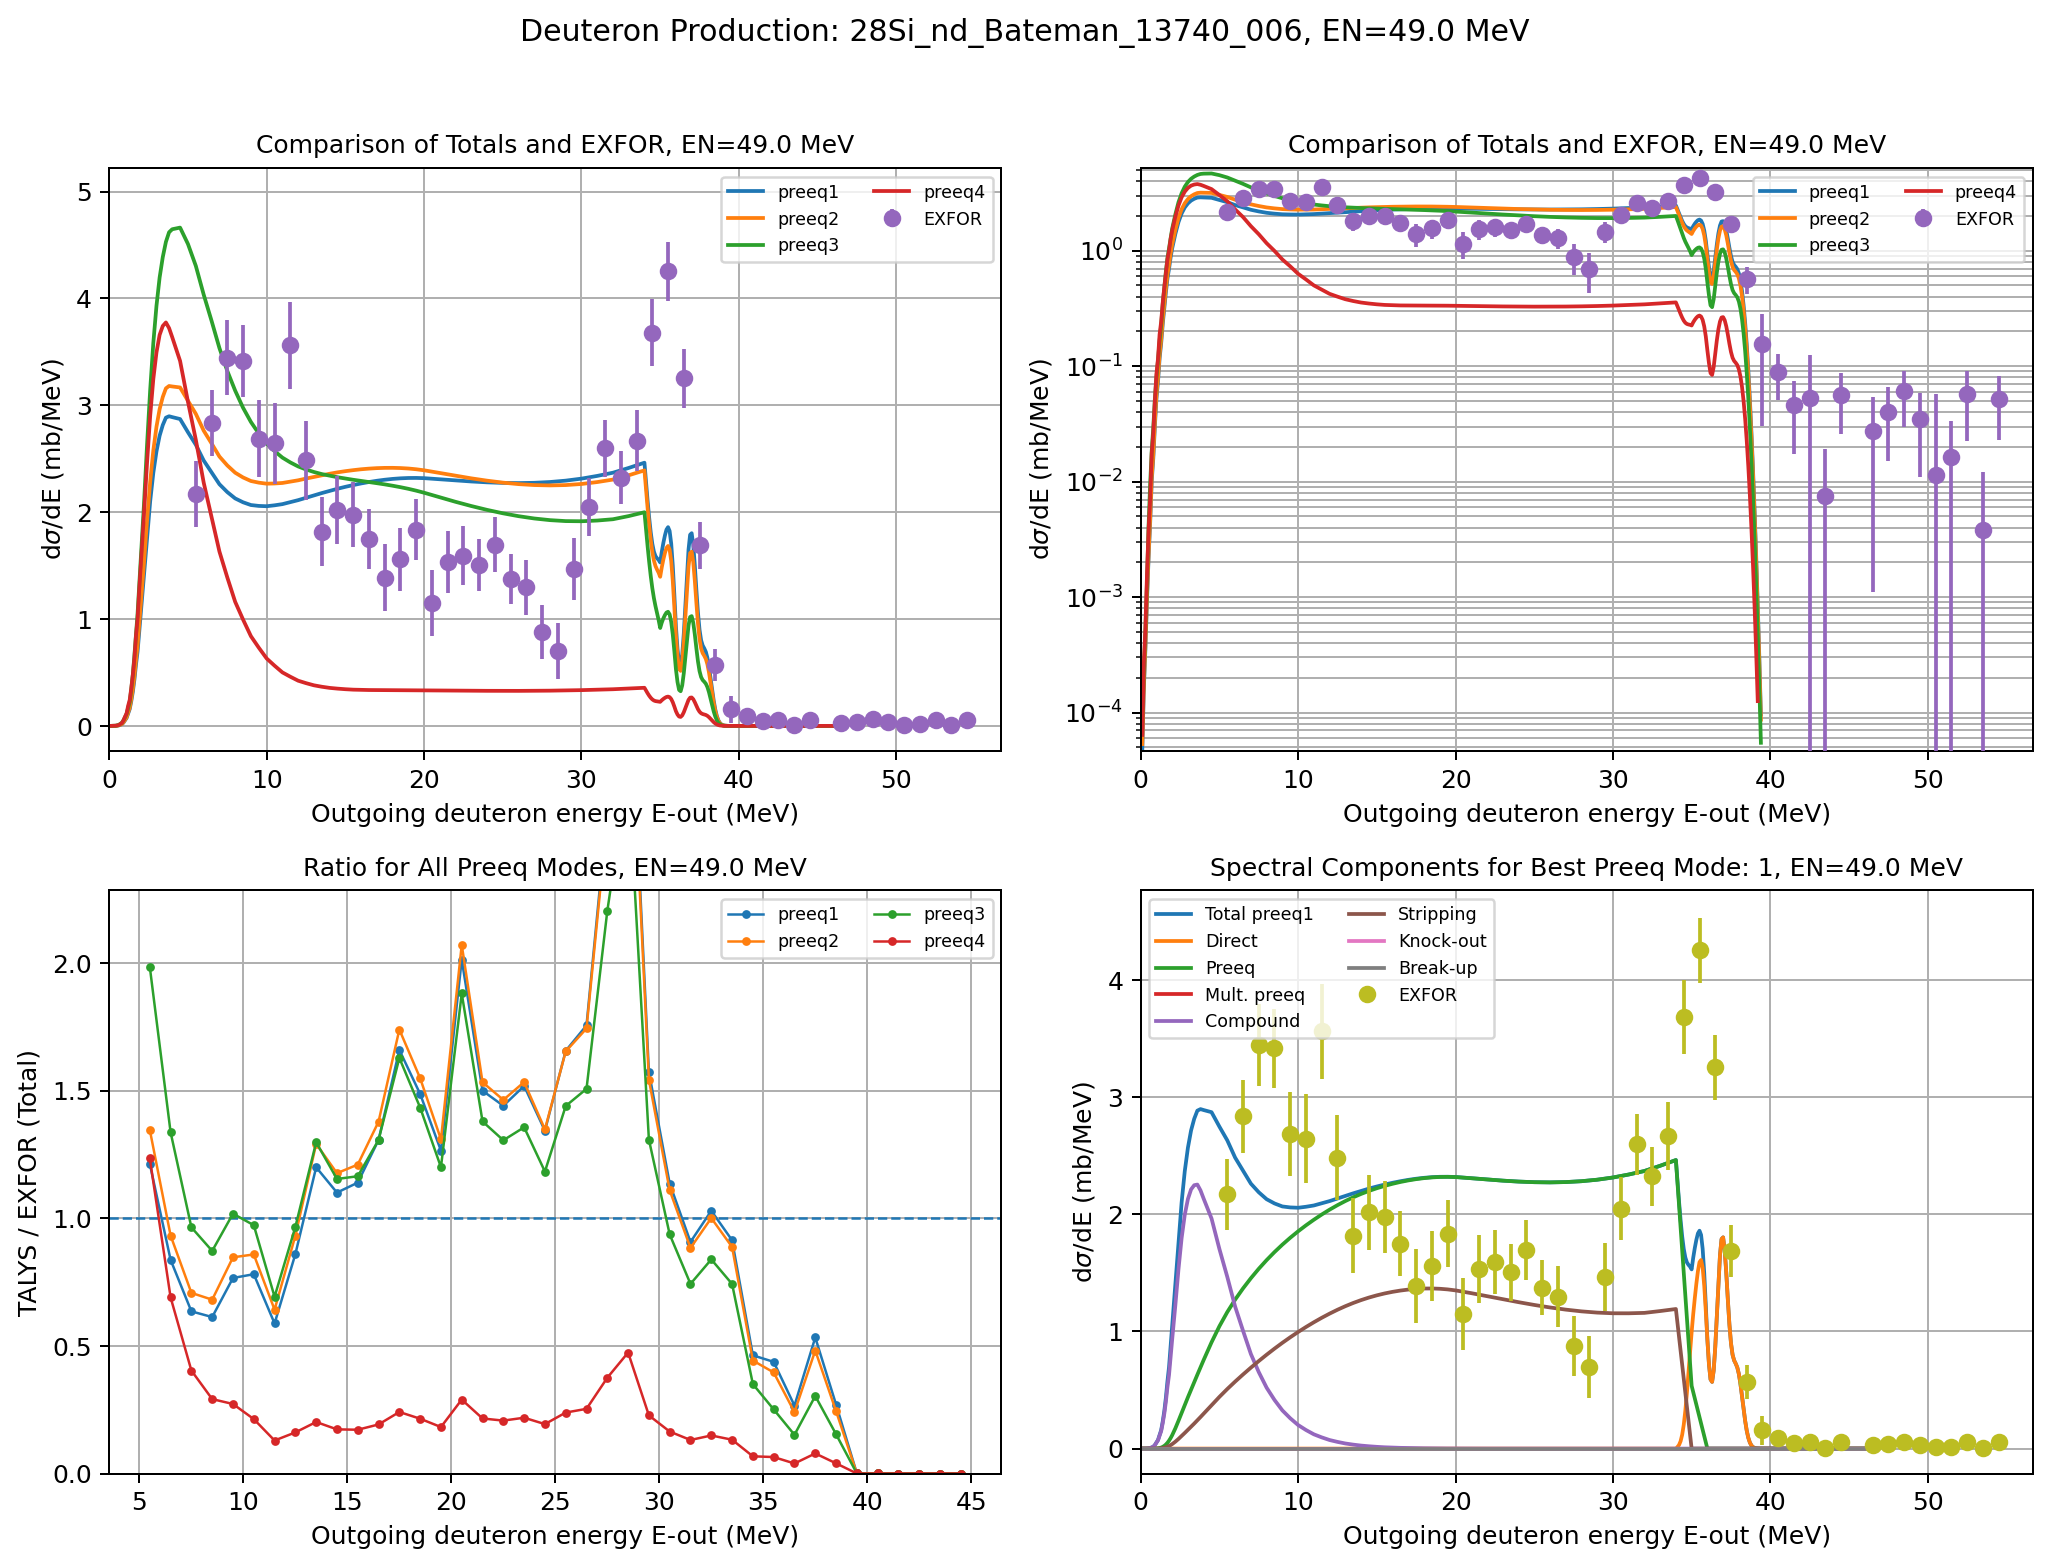
\includegraphics[width=\textwidth]{Images/EN49.0_00_2x2_diagnostics_28Si_nd_Bateman_13740_006.png}
    \caption{Diagnostic panels for deuteron production on \ce{^{28}Si} using the Bateman EXFOR dataset 13740.006 at $E_n=49.0$ MeV. The decomposition panel corresponds to the selected mode, \texttt{preeqmode=1}.}
    \label{fig:bateman-en49-d-diagnostics}
\end{figure}

At $E_n=49.0$ MeV, shown in \cref{fig:bateman-en49-d-diagnostics}, the overlap between TALYS and EXFOR becomes more evident across the main part of the measured spectrum. The spectra still contain narrow structures and the experimental uncertainties remain sizeable, but the general trend is reproduced better than at lower incident energies.

The selected mode changes to \texttt{preeqmode=1}. The ratio panel shows that, over much of the measured interval, this mode remains closer to $R\simeq 1$ than the alternatives. A large ratio peak above 3 is still present, showing that the agreement is not uniform. As in the lower-energy cases, the ratio eventually drops toward $R\simeq 0$, but only at higher $E_{\mathrm{out}}$. This means that the effective high-energy cut-off in the TALYS prediction is shifted to higher outgoing energy as the incident energy increases.

Overall, for the Bateman deuteron-production dataset, the preferred mode is case-dependent: \texttt{preeqmode=4} at $E_n=28.0$ MeV, \texttt{preeqmode=2} at $E_n=41.0$ MeV, and \texttt{preeqmode=1} at $E_n=49.0$ MeV. This confirms that, for deuteron emission, the model choice is controlled mainly by the shoulder and high-energy-tail behaviour rather than by the low-energy evaporation peak.
 % This file currently contains the deuteron results. Rename it to deuteron_results.tex if you prefer.
\subsection{Methods}
The package \verb+NetworkX+ offers the function \verb+watts_strogatz_graph+ to make a Watts-Strogatz graph. 
Conveniently, this function takes $N$, $k$ and $p$ as arguments. Using this function we created all graphs for this exercise.
Thus, to run our code, the package \verb+NetworkX+ needs to be installed.
We used the suggested values of $N=200$ and $k=6$ for all graphs, but will run several simulations while varying $p$. The different values of the probability will be picked from the following list: $[0.0, 0.001, 0.003, 0.01, 0.03, 0.10, 0.30, 1.0]$.

The graph can also be plotted using the \texttt{draw\_circular()} or \texttt{draw\_networkx()}, which takes in the Watts-Strogatz graph and generates a circular plot or an arbitrary plot. Typically, the graph is shown as a circle and this is how it was presented in figure \ref{fig:WScircleplot}.

\subsubsection{Degrees and degree distribution}

To study how the distribution of the degree $d_i$ of a Watts-Strogatz graph changes by varying $p$ value a pyton script \verb+WS_1_degrees.py+ was written. It can be run using the command \verb+python3 WS_1_degrees.py+. The script creates a Watts-Strogatz graphs with fixed parameters $N=200$ and $k=6$ and a variable parameter $p$ that is varied from $0.0$ to $1.0$. For each $p$ value 1000 separate instances of the graph are created and the degree of each node is studied. Then the results over the 1000 instances are averaged and so are created degree distributions for each $p$ value. Finally histograms are created for each $p$ value and saved as a file \verb+WS_1_degrees.png+. The script utilizes the following Python packages: NetworkX, NumPy and matplotlib.

\input{texfiles/connected_method.tex}

\subsubsection{Diameter and average path length}

The same Python package \texttt{NetworkX} has many useful functions. Once the Watts-Strogatz graph has been generated using the \texttt{nx.watts\_strogatz\_graph} function, the following functions are then used: \texttt{nx.diameter()} and \texttt{nx.average\_shortest\_path\_length()}. As the names of the functions indicate, the \texttt{nx.diameter()} returns the diameter (as defined in equation \ref{eq:WSdiameter}) and the latter function computes the average path length (as defined in equation \ref{eq:WSavgshortestpath}). In the case of an disconnected graph, the diameter and average path length would be computed for the largest connected component of the graph.

The computations are repeated 1000 times for each value of $p$, with a new seed each times. For every iteration, a new graph is generated and the relevant values are saved in a \texttt{NumPy}-array. This will then be used to produce the results visible in section \ref{sec:WS_Diam&ASPL_result}.


\subsubsection{Clustering Coefficient}
The package \verb+NetworkX+ has the function \verb+clustering+, with which the clustering of a graph can be calculated. 
The average shortest path length is calculated using the function \verb+nx.average_shortest_path_length+.
In our code we iterate over the different values of $p$ ($p$ = [0, 0.001, 0.003, 0.01, 0.03, 0.1, 0.3, 1]) as well as 1000 different seeds (1-1000). 
This way the results of our calculations are reproducible. 

The function \verb+networkx.clustering+ outputs a dictionary with the local clustering coefficients of each node. 
For each graph, we take the average of these local clustering coefficients and append them to a list for the current p. 
After iterating over all 1000 seeds, the average for the current p-value is taken and saved to another list.
Additionally, the standard deviation of the clustering coefficients is calculated using numpy and saved to yet another list. 
Then we continue with the next value of p. 

After iterating over all p values, the averaged values and their standard deviation are plotted using \verb+plt.errorbar+. 
All values are normalised by the value at $p=0$.
The whole code is timed, as we were afraid it would take too long to execute it.

To reproduce Figure \ref{fig:cluster_coeff} you need to run \verb+clustering_coeff.py+.
The required packages are \verb+NetworkX+, \verb+numpy+, \verb+matplotlib+ and \verb+time+.



\section{Conclusion}
\subsection{Synthesis}

\begin{itemize}
    \item For which values of $p$ do you see high clustering together with short average path length?
    
We can see an especially large difference between clustering and average shortest path length at $p=0.01, 0.03, 0.1$. The clustering for these values values of p is roughly
at $0.95$, $ 0.9$ and $0.75$, while the average shortest path length has already decreased to $0.55$, $0.4$ and $0.25$ (all values are normalised by the value at p=0).

    \item How variable are the Watts--Strogatz statistics across different random realizations with the same $p$?
    
Looking at Figure \ref{fig:cluster_coeff}, the error bars and with this the standard deviation of the values highly depends on the p value.
For very low p, the standard deviation of the average shortest path length is very high. 
The low probability of rewiring an edge leads to graphs with very different shortest paths: No rewiring can happen, which leaves the shortest path length untouched. 
One or a few very efficient shortcuts, however, can decrease the shortest path length very quickly. We assume this is where the large standard deviation comes from. 
At higher values of p the graphs get more and more random and the statistical process of rewiring so many edges distributes them so that the shortest paths are very similar in all graphs.
For the clustering coefficient we see the highest uncertainty for the higher p values. 
At low p values only a few connections will be rewired and only by this amount can the clustering coefficient change. 
When more edges get rewired more connections between neighbours are broken up. The clustering will depend a lot on how exactly the connections are rewired.
At $p=1$ the standard deviation of the clustering is again very small. Again, this is due to the high statistics when rewiring each edge. 

   \item In the Markov-chain experiment, how does the second-largest eigenvalue modulus affect the observed convergence speed?

The second-largest eigenvalue modulus \(\mu\) determines the speed at which the Markov chain approaches the stationary distribution. When \(\mu\) is smaller, the term \(\mu^t\) decreases faster, so the distance between \(x_t\) and \(\pi\) becomes small in fewer steps. When \(\mu\) is closer to \(1\), \(\mu^t\) decreases more slowly, so convergence takes longer.

This can be seen in the numerical results. The original matrix \(P_0\) has the smallest value of \(\mu\), and it converges the fastest. For the lazy matrices, increasing \(\alpha\) moves the nontrivial eigenvalues closer to \(1\), which therefore increases \(\mu\). As a result, the convergence rate increases like this, \(P_{0.8}\) \rightarrow \(P_{0.5}\) \rightarrow \(P_0\). The observed convergence speed agrees with the spectral prediction, in the theoretical section, larger \(\mu\) means slower convergence.

\item Why is the spectral gap \(g = 1 - \mu\) a more direct predictor of convergence speed than visual inspection of the entries of \(P\)?

The spectral gap \(g = 1 - \mu\) is a more direct predictor of convergence speed because it measures how quickly the slowest non-stationary component of the distribution decays. The entries of \(P\) show the one-step transition probabilities, but they do not directly show how repeated multiplication by \(P\) behaves over many time steps. Two matrices can look similar when analysed entry by entry, but having different eigenvalues, can result in very different long-term convergence speeds.

The spectral gap is able to summarize this long-term behaviour. If \(g\) is large, then \(\mu\) is far from \(1\), so the error decreases quickly. If \(g\) is small, then \(\mu\) is close to \(1\), so the error decreases slowly. For this reason, \(g\) is more informative and precise.

\item What are the limitations of using only one graph realization for each value of \(p\), or only one initial condition for the Markov chain?

Using only one graph for each value of \(p\) is limited since the Watts - Strogatz model is random for \(p>0\). A single graph may not represent the typical behaviour for that value of \(p\), especially for small \(p\), where the presence or absence of only a few shortcuts can strongly affect the average path length.

Similarly, using only one initial condition for the Markov chain is limited because the observed convergence can depend on where the chain starts. Some initial distributions may have a larger component in the slowest-decaying eigenvector direction, while others may have a smaller one. Even if one initial condition is enough to illustrate the spectral mechanism, it does not fully describe all possible convergence behaviours. For a more complete experiment, it would be needed several initial states to make a direct comparison and conclusion of the overall trend.

Overall, scientific research should be done varying all the different parameters that can affect the system at play so a comparison can be done and a long-term behaviour can be studied.
\end{itemize}


\newpage
\section{Use of LLM tools}

For writing the code and report for the part about Watts-Strogatz networks, no LLM was involved.

For writing the parts about the Markov chain, both code and in the report, no LLM was involved.

\newpage
\section*{Files submitted}
\begin{itemize}
% for markov chain
	\item \texttt{numerics\_mc.py}
	\item \texttt{Watts\_Strogatz\_diameter\_ASPL.py}
	\item \texttt{clustering\_coeff.py}
	\item \texttt{WS\_1\_degrees.py}
	\item \texttt{WS\_2\_connected.py}
\end{itemize}




\subsection{Synthesis}

\begin{itemize}
    \item For which values of $p$ do you see high clustering together with short average path length?
    
We can see an especially large difference between clustering and average shortest path length at $p=0.01, 0.03, 0.1$. The clustering for these values values of p is roughly
at $0.95$, $ 0.9$ and $0.75$, while the average shortest path length has already decreased to $0.55$, $0.4$ and $0.25$ (all values are normalised by the value at p=0).

    \item How variable are the Watts--Strogatz statistics across different random realizations with the same $p$?
    
Looking at Figure \ref{fig:cluster_coeff}, the error bars and with this the standard deviation of the values highly depends on the p value.
For very low p, the standard deviation of the average shortest path length is very high. 
The low probability of rewiring an edge leads to graphs with very different shortest paths: No rewiring can happen, which leaves the shortest path length untouched. 
One or a few very efficient shortcuts, however, can decrease the shortest path length very quickly. We assume this is where the large standard deviation comes from. 
At higher values of p the graphs get more and more random and the statistical process of rewiring so many edges distributes them so that the shortest paths are very similar in all graphs.
For the clustering coefficient we see the highest uncertainty for the higher p values. 
At low p values only a few connections will be rewired and only by this amount can the clustering coefficient change. 
When more edges get rewired more connections between neighbours are broken up. The clustering will depend a lot on how exactly the connections are rewired.
At $p=1$ the standard deviation of the clustering is again very small. Again, this is due to the high statistics when rewiring each edge. 

   \item In the Markov-chain experiment, how does the second-largest eigenvalue modulus affect the observed convergence speed?

The second-largest eigenvalue modulus \(\mu\) determines the speed at which the Markov chain approaches the stationary distribution. When \(\mu\) is smaller, the term \(\mu^t\) decreases faster, so the distance between \(x_t\) and \(\pi\) becomes small in fewer steps. When \(\mu\) is closer to \(1\), \(\mu^t\) decreases more slowly, so convergence takes longer.

This can be seen in the numerical results. The original matrix \(P_0\) has the smallest value of \(\mu\), and it converges the fastest. For the lazy matrices, increasing \(\alpha\) moves the nontrivial eigenvalues closer to \(1\), which therefore increases \(\mu\). As a result, the convergence rate increases like this, \(P_{0.8}\) \rightarrow \(P_{0.5}\) \rightarrow \(P_0\). The observed convergence speed agrees with the spectral prediction, in the theoretical section, larger \(\mu\) means slower convergence.

\item Why is the spectral gap \(g = 1 - \mu\) a more direct predictor of convergence speed than visual inspection of the entries of \(P\)?

The spectral gap \(g = 1 - \mu\) is a more direct predictor of convergence speed because it measures how quickly the slowest non-stationary component of the distribution decays. The entries of \(P\) show the one-step transition probabilities, but they do not directly show how repeated multiplication by \(P\) behaves over many time steps. Two matrices can look similar when analysed entry by entry, but having different eigenvalues, can result in very different long-term convergence speeds.

The spectral gap is able to summarize this long-term behaviour. If \(g\) is large, then \(\mu\) is far from \(1\), so the error decreases quickly. If \(g\) is small, then \(\mu\) is close to \(1\), so the error decreases slowly. For this reason, \(g\) is more informative and precise.

\item What are the limitations of using only one graph realization for each value of \(p\), or only one initial condition for the Markov chain?

Using only one graph for each value of \(p\) is limited since the Watts - Strogatz model is random for \(p>0\). A single graph may not represent the typical behaviour for that value of \(p\), especially for small \(p\), where the presence or absence of only a few shortcuts can strongly affect the average path length.

Similarly, using only one initial condition for the Markov chain is limited because the observed convergence can depend on where the chain starts. Some initial distributions may have a larger component in the slowest-decaying eigenvector direction, while others may have a smaller one. Even if one initial condition is enough to illustrate the spectral mechanism, it does not fully describe all possible convergence behaviours. For a more complete experiment, it would be needed several initial states to make a direct comparison and conclusion of the overall trend.

Overall, scientific research should be done varying all the different parameters that can affect the system at play so a comparison can be done and a long-term behaviour can be studied.
\end{itemize}

\clearpage
\appendix

\section{Additional Diagnostic Figures}

This appendix includes the remaining diagnostic figures generated with the same 2x2 format as the figures discussed in the main text.

\subsection{Additional Proton Production Figures}

\subsubsection*{\ce{^{28}Si}, Benck, 22807.012}

\begin{figure}[H]
    \centering
    
\includegraphics[width=\textwidth]{Images/Proton/Benck/proton/EN30.0_00_2x2_diagnostics_28Si_np_Benck_22807_012.png}
    \caption{Diagnostic comparison for proton production from \ce{^{28}Si}, Benck dataset 22807.012, at $E_n=30.0$ MeV.}
    \label{fig:app-benck-en30-p-diagnostics}
\end{figure}

\begin{figure}[H]
    \centering
    
\includegraphics[width=\textwidth]{Images/Proton/Benck/proton/EN35.0_00_2x2_diagnostics_28Si_np_Benck_22807_012.png}
    \caption{Diagnostic comparison for proton production from \ce{^{28}Si}, Benck dataset 22807.012, at $E_n=35.0$ MeV.}
    \label{fig:app-benck-en35-p-diagnostics}
\end{figure}

\begin{figure}[H]
    \centering
    
\includegraphics[width=\textwidth]{Images/Proton/Benck/proton/EN45.0_00_2x2_diagnostics_28Si_np_Benck_22807_012.png}
    \caption{Diagnostic comparison for proton production from \ce{^{28}Si}, Benck dataset 22807.012, at $E_n=45.0$ MeV.}
    \label{fig:app-benck-en45-p-diagnostics}
\end{figure}

\subsubsection*{\ce{^{28}Si}, Bateman, 13740.005}



\begin{figure}[H]
    \centering
    
\includegraphics[width=\textwidth]{Images/Proton/Bateman/proton/EN30.0_00_2x2_diagnostics_28Si_np_Bateman_13740_005.png}
    \caption{Diagnostic comparison for proton production from \ce{^{28}Si}, Bateman dataset 13740.005, at $E_n=30.0$ MeV.}
    \label{fig:app-bateman-en30-p-diagnostics}
\end{figure}

\begin{figure}[H]
    \centering
    
\includegraphics[width=\textwidth]{Images/Proton/Bateman/proton/EN35.0_00_2x2_diagnostics_28Si_np_Bateman_13740_005.png}
    \caption{Diagnostic comparison for proton production from \ce{^{28}Si}, Bateman dataset 13740.005, at $E_n=35.0$ MeV.}
    \label{fig:app-bateman-en35-p-diagnostics}
\end{figure}

\begin{figure}[H]
    \centering
    
\includegraphics[width=\textwidth]{Images/Proton/Bateman/proton/EN45.0_00_2x2_diagnostics_28Si_np_Bateman_13740_005.png}
    \caption{Diagnostic comparison for proton production from \ce{^{28}Si}, Bateman dataset 13740.005, at $E_n=45.0$ MeV.}
    \label{fig:app-bateman-en45-p-diagnostics}
\end{figure}

\subsubsection*{\ce{^{56}Fe}, Slypen, 22884.015}

\begin{figure}[H]
    \centering
    
\includegraphics[width=\textwidth]{Images/Proton/Slypen/proton/EN41.0_00_2x2_diagnostics_56Fe_np_Slypen_22884_015.png}
    \caption{Diagnostic comparison for proton production from \ce{^{56}Fe}, Slypen dataset 22884.015, at $E_n=41.0$ MeV.}
    \label{fig:app-slypen-en41-p-diagnostics}
\end{figure}

\begin{figure}[H]
    \centering
    
\includegraphics[width=\textwidth]{Images/Proton/Slypen/proton/EN45.0_00_2x2_diagnostics_56Fe_np_Slypen_22884_015.png}
    \caption{Diagnostic comparison for proton production from \ce{^{56}Fe}, Slypen dataset 22884.015, at $E_n=45.0$ MeV.}
    \label{fig:app-slypen-en45-p-diagnostics}
\end{figure}

\begin{figure}[H]
    \centering
    
\includegraphics[width=\textwidth]{Images/Proton/Slypen/proton/EN53.5_00_2x2_diagnostics_56Fe_np_Slypen_22884_015.png}
    \caption{Diagnostic comparison for proton production from \ce{^{56}Fe}, Slypen dataset 22884.015, at $E_n=53.5$ MeV.}
    \label{fig:app-slypen-en53p5-p-diagnostics}
\end{figure}

\begin{figure}[H]
    \centering
    
\includegraphics[width=\textwidth]{Images/Proton/Slypen/proton/EN62.7_00_2x2_diagnostics_56Fe_np_Slypen_22884_015.png}
    \caption{Diagnostic comparison for proton production from \ce{^{56}Fe}, Slypen dataset 22884.015, at $E_n=62.7$ MeV.}
    \label{fig:app-slypen-en62p7-p-diagnostics}
\end{figure}

\subsubsection*{\ce{^{52}Cr}, Grimes, 22807.027}

\begin{figure}[H]
    \centering
    
\includegraphics[width=\textwidth]{Images/Proton/Grimes/EN14.8_00_2x2_diagnostics_52Cr_np_Grimes_22807_027.png}
    \caption{Diagnostic comparison for proton production from \ce{^{52}Cr}, Grimes dataset 22807.027, at $E_n=14.8$ MeV.}
    \label{fig:app-grimes-en14p8-p-diagnostics}
\end{figure}

\subsubsection*{\ce{^{56}Fe}, Kokoo, 22467.026}

\begin{figure}[H]
    \centering
    
\includegraphics[width=\textwidth]{Images/Proton/Kokoo/EN14.1_00_2x2_diagnostics_56Fe_np_Kokoo_22467_026.png}
    \caption{Diagnostic comparison for proton production from \ce{^{56}Fe}, Kokoo dataset 22467.026, at $E_n=14.1$ MeV.}
    \label{fig:app-kokoo-en14p1-p-diagnostics}
\end{figure}

\subsection{Additional Deuteron Production Figures}


\subsubsection*{\ce{^{28}Si}, Benck, 22807.027}

\begin{figure}[H]
    \centering
    
\includegraphics[width=\textwidth]{Images/Deuteron/Benck/deuteron/EN34.5_00_2x2_diagnostics_28Si_nd_Benck_22807_027.png}
    \caption{Diagnostic comparison for deuteron production from \ce{^{28}Si}, Benck dataset 22807.027, at $E_n=34.5$ MeV.}
    \label{fig:app-benck-en34p5-d-diagnostics}
\end{figure}

\subsubsection*{\ce{^{28}Si}, Bateman, 13740.006}

\begin{figure}[H]
    \centering
    
\includegraphics[width=\textwidth]{Images/Deuteron/Bateman/deuteron/EN33.0_00_2x2_diagnostics_28Si_nd_Bateman_13740_006.png}
    \caption{Diagnostic comparison for deuteron production from \ce{^{28}Si}, Bateman dataset 13740.006, at $E_n=33.0$ MeV.}
    \label{fig:app-bateman-en33-d-diagnostics}
\end{figure}



\bibliographystyle{plainnat}
\bibliography{main}

\end{document}
